% Meridian project report. All results are macros/tables generated by
% scripts/build_report_tex.py from the saved results files; do not type numbers here.
\documentclass[11pt,a4paper]{article}

\usepackage[T1]{fontenc}
\usepackage[utf8]{inputenc}
\usepackage{libertinus}
\usepackage[scaled=0.92]{inconsolata}
\usepackage{amsmath,amssymb,mathtools}
\usepackage[a4paper,margin=2.3cm,headheight=14pt]{geometry}
\usepackage{microtype}
\usepackage{booktabs,tabularx,array,colortbl,multirow}
\usepackage[table]{xcolor}
\usepackage{graphicx,float}
\usepackage[font=small,labelfont=bf,skip=4pt]{caption}
\usepackage{enumitem}
\usepackage{algorithm}
\usepackage{algpseudocode}
\usepackage{fancyhdr}
\usepackage{titlesec}
\usepackage[most]{tcolorbox}
\usepackage[hidelinks,bookmarksnumbered]{hyperref}
\usepackage[nameinlink]{cleveref}

\definecolor{accent}{HTML}{1D4E89}
\definecolor{good}{HTML}{E3F2E8}
\definecolor{bad}{HTML}{FBEAEA}
\definecolor{muted}{HTML}{52606D}
\hypersetup{colorlinks=true,linkcolor=accent,urlcolor=accent,citecolor=accent}

\titleformat{\section}{\Large\bfseries\color{accent}}{\thesection}{0.8em}{}
\titleformat{\subsection}{\large\bfseries}{\thesubsection}{0.7em}{}
\setlist{itemsep=2pt,topsep=4pt}
\renewcommand{\arraystretch}{1.12}

\pagestyle{fancy}
\fancyhf{}
\lhead{\small\color{muted}Meridian --- project status report}
\rhead{\small\color{muted}\today}
\cfoot{\small\thepage}
\renewcommand{\headrulewidth}{0.3pt}

\newtcolorbox{keybox}[1][]{colback=accent!4,colframe=accent,boxrule=0.6pt,arc=1pt,
  left=6pt,right=6pt,top=4pt,bottom=4pt,fonttitle=\bfseries,title=#1}
\newtcolorbox{warnbox}[1][]{colback=orange!5,colframe=orange!70!black,boxrule=0.6pt,arc=1pt,
  left=6pt,right=6pt,top=4pt,bottom=4pt,fonttitle=\bfseries,title=#1}

% generated by scripts/build_report_tex.py -- do not edit
\newcommand{\AblMOne}{0.3432}
\newcommand{\AblMThree}{0.3477}
\newcommand{\AblMTwo}{0.3430}
\newcommand{\AblMZero}{0.3404}
\newcommand{\AblRuntimeMin}{41}
\newcommand{\AblSeeds}{3}
\newcommand{\AssetBest}{QQQ}
\newcommand{\AssetBestPct}{$-12.6\%$}
\newcommand{\AssetWorst}{USDJPY}
\newcommand{\AssetWorstPct}{$-1.1\%$}
\newcommand{\BreadthMCI}{[-12.4, -2.1]}
\newcommand{\BreadthMP}{0.002}
\newcommand{\BreadthMPct}{$-7.1\%$}
\newcommand{\DataEnd}{2026-07-31}
\newcommand{\DataStart}{2007-01-01}
\newcommand{\DevDates}{1,901}
\newcommand{\DevEnd}{2018-12-31}
\newcommand{\DevMPct}{$-8.8\%$}
\newcommand{\DevStart}{2012-06-14}
\newcommand{\EmbargoDays}{22}
\newcommand{\Epochs}{8}
\newcommand{\FirstYear}{2012}
\newcommand{\Folds}{12}
\newcommand{\FwdCommit}{108f349}
\newcommand{\FwdFirstOrigin}{2026-10-30}
\newcommand{\FwdFrozen}{2026-11-01 16:19:03 UTC}
\newcommand{\FwdLastOrigin}{2026-11-02}
\newcommand{\FwdLogged}{26}
\newcommand{\FwdOrigins}{2}
\newcommand{\FwdPct}{$+13.0\%$}
\newcommand{\FwdPre}{26}
\newcommand{\FwdQH}{0.3201}
\newcommand{\FwdQM}{0.3617}
\newcommand{\FwdScoredAt}{2026-11-03 08:44:08 UTC}
\newcommand{\FwdScoredDates}{1}
\newcommand{\FwdScoredN}{11}
\newcommand{\FwdScoredOrigin}{2026-10-30}
\newcommand{\FwdTrainRows}{54,481}
\newcommand{\FwdTrainThrough}{2026-10-29}
\newcommand{\GitAhead}{5}
\newcommand{\GitHead}{0a6cfcc}
\newcommand{\GitMain}{ab041b0}
\newcommand{\HFiveP}{$<$0.001}
\newcommand{\HFivePct}{$-9.6\%$}
\newcommand{\HHFiveP}{0.203}
\newcommand{\HHOne}{$-3.1\%$}
\newcommand{\HHOneP}{0.076}
\newcommand{\HHTwoP}{0.369}
\newcommand{\HTwentyTwoP}{0.356}
\newcommand{\HTwentyTwoPct}{$-0.9\%$}
\newcommand{\HitMax}{68.3\%}
\newcommand{\HitMin}{62.3\%}
\newcommand{\HoldAssets}{11}
\newcommand{\HoldDates}{2,168}
\newcommand{\HoldEnd}{2026-06-29}
\newcommand{\HoldRows}{20,906}
\newcommand{\HoldStart}{2019-01-01}
\newcommand{\LastYear}{2026}
\newcommand{\MacroEnd}{2026-07-28}
\newcommand{\MacroStart}{2007-01-02}
\newcommand{\MinTrainDays}{1260}
\newcommand{\NClipped}{469}
\newcommand{\NScripts}{68}
\newcommand{\NStale}{36}
\newcommand{\NTests}{11}
\newcommand{\NWLag}{7}
\newcommand{\PowerEighty}{451}
\newcommand{\PowerEightyYears}{1.8}
\newcommand{\PowerFifty}{197}
\newcommand{\PowerFiftyMonths}{9}
\newcommand{\RawComboCI}{[-9.5, -4.9]}
\newcommand{\RawComboPct}{$-7.0\%$}
\newcommand{\RawHARQ}{0.3249}
\newcommand{\RawHARcalPct}{$+1.3\%$}
\newcommand{\RawMCI}{[-9.7, -4.5]}
\newcommand{\RawMCIHi}{$-4.5\%$}
\newcommand{\RawMP}{$<$0.001}
\newcommand{\RawMPct}{$-6.8\%$}
\newcommand{\RegCalmPct}{$-4.1\%$}
\newcommand{\RegNormalPct}{$-5.2\%$}
\newcommand{\RegStressPct}{$-14.1\%$}
\newcommand{\Seeds}{5}
\newcommand{\ShareDay}{61.2\%}
\newcommand{\ShareSixtyThree}{96.5\%}
\newcommand{\ShareTwenty}{86.6\%}
\newcommand{\ShareTwoFiftyTwo}{100.0\%}
\newcommand{\TCC}{11}
\newcommand{\TCCFive}{11}
\newcommand{\TCCOne}{11}
\newcommand{\TCCTwo}{11}
\newcommand{\TDQ}{10}
\newcommand{\TDQFive}{9}
\newcommand{\TDQOne}{10}
\newcommand{\TDQTwo}{10}
\newcommand{\TDevHAR}{-3.7832}
\newcommand{\TDevSel}{-3.7753}
\newcommand{\TESR}{0.98}
\newcommand{\TFZ}{-0.1218}
\newcommand{\TFZCI}{[-0.1533, -0.0949]}
\newcommand{\TFZP}{$<$0.001}
\newcommand{\TGNOneViol}{1.80\%}
\newcommand{\THSOne}{$+26.3\%$}
\newcommand{\THarDQ}{8}
\newcommand{\THarEVTDQ}{7}
\newcommand{\TKupFive}{11}
\newcommand{\TKupOne}{11}
\newcommand{\TKupTwo}{11}
\newcommand{\TRMOneViol}{2.10\%}
\newcommand{\TVFive}{$-5.1\%$}
\newcommand{\TVOne}{$-9.2\%$}
\newcommand{\TVOneCI}{[-12.7, -5.9]}
\newcommand{\TVOneP}{$<$0.001}
\newcommand{\TVTwo}{$-7.4\%$}
\newcommand{\TViolFive}{4.95\%}
\newcommand{\TViolOne}{0.96\%}
\newcommand{\TViolTwo}{2.49\%}
\newcommand{\TailDates}{2,168}
\newcommand{\TailEVTu}{0.90}
\newcommand{\TailGamma}{0.005}
\newcommand{\TailHS}{500}
\newcommand{\TailRef}{GJR-GARCH + FHS}
\newcommand{\TailRefit}{21}
\newcommand{\TailRows}{20,906}
\newcommand{\TailRuntime}{99}
\newcommand{\TailSel}{Meridian + EVT}
\newcommand{\TailZMin}{250}
\newcommand{\TailZWin}{1000}
\newcommand{\TestDays}{378}
\newcommand{\VComboCI}{[-12.4, -5.2]}
\newcommand{\VComboP}{$<$0.001}
\newcommand{\VComboPct}{$-8.2\%$}
\newcommand{\VComboQ}{0.3022}
\newcommand{\VComboWon}{11}
\newcommand{\VEGARCHCI}{[+8.1, +16.8]}
\newcommand{\VEGARCHP}{1.000}
\newcommand{\VEGARCHPct}{$+12.2\%$}
\newcommand{\VEGARCHQ}{0.3695}
\newcommand{\VEGARCHWon}{0}
\newcommand{\VEWMACI}{[+7.9, +21.8]}
\newcommand{\VEWMAP}{1.000}
\newcommand{\VEWMAPct}{$+14.1\%$}
\newcommand{\VEWMAQ}{0.3758}
\newcommand{\VEWMAWon}{0}
\newcommand{\VGARCHCI}{[+11.0, +18.6]}
\newcommand{\VGARCHP}{1.000}
\newcommand{\VGARCHPct}{$+14.9\%$}
\newcommand{\VGARCHQ}{0.3782}
\newcommand{\VGARCHWon}{0}
\newcommand{\VGJRCI}{[+9.9, +18.9]}
\newcommand{\VGJRP}{1.000}
\newcommand{\VGJRPct}{$+14.1\%$}
\newcommand{\VGJRQ}{0.3758}
\newcommand{\VGJRWon}{0}
\newcommand{\VHARLGBMCI}{[-9.3, -3.1]}
\newcommand{\VHARLGBMP}{$<$0.001}
\newcommand{\VHARLGBMPct}{$-5.7\%$}
\newcommand{\VHARLGBMQ}{0.3105}
\newcommand{\VHARLGBMWon}{10}
\newcommand{\VHARQ}{0.3292}
\newcommand{\VHARXCI}{[-7.7, -2.9]}
\newcommand{\VHARXP}{$<$0.001}
\newcommand{\VHARXPct}{$-5.0\%$}
\newcommand{\VHARXQ}{0.3126}
\newcommand{\VHARXWon}{10}
\newcommand{\VLGBMCI}{[-9.3, -2.5]}
\newcommand{\VLGBMP}{$<$0.001}
\newcommand{\VLGBMPct}{$-5.3\%$}
\newcommand{\VLGBMQ}{0.3118}
\newcommand{\VLGBMWon}{10}
\newcommand{\VLHARCI}{[-5.4, -0.5]}
\newcommand{\VLHARP}{0.011}
\newcommand{\VLHARPct}{$-2.7\%$}
\newcommand{\VLHARQ}{0.3204}
\newcommand{\VLHARWon}{10}
\newcommand{\VMCI}{[-11.3, -4.7]}
\newcommand{\VMP}{$<$0.001}
\newcommand{\VMPct}{$-7.5\%$}
\newcommand{\VMQ}{0.3045}
\newcommand{\VMWon}{11}
\newcommand{\VRFCI}{[-6.8, -1.4]}
\newcommand{\VRFP}{$<$0.001}
\newcommand{\VRFPct}{$-3.7\%$}
\newcommand{\VRFQ}{0.3171}
\newcommand{\VRFWon}{11}
\newcommand{\VRWCI}{[+12.9, +24.7]}
\newcommand{\VRWP}{1.000}
\newcommand{\VRWPct}{$+18.0\%$}
\newcommand{\VRWQ}{0.3884}
\newcommand{\VRWWon}{0}
\newcommand{\VRidgeCI}{[-8.7, -2.1]}
\newcommand{\VRidgeP}{$<$0.001}
\newcommand{\VRidgePct}{$-4.9\%$}
\newcommand{\VRidgeQ}{0.3132}
\newcommand{\VRidgeWon}{9}
\newcommand{\VTMCI}{[+0.3, +6.1]}
\newcommand{\VTMP}{0.957}
\newcommand{\VTMPct}{$+3.0\%$}
\newcommand{\VTMQ}{0.3392}
\newcommand{\VTMWon}{3}
\newcommand{\VolRunCommit}{ab041b0}
\newcommand{\VolRuntimeMin}{18}
\newcommand{\WorstYear}{2026}
\newcommand{\WorstYearPct}{$+0.04\%$}
\newcommand{\YearsTotal}{15}
\newcommand{\YearsWon}{14}


\begin{document}

% ------------------------------------------------------------------ title
\begin{titlepage}
\centering
\vspace*{2.2cm}
{\Huge\bfseries\color{accent} Meridian\par}
\vspace{0.5cm}
{\Large A state-space neural forecaster of daily financial volatility:\\[2pt]
audited benchmark, tail-risk evaluation and forward test\par}
\vspace{1.2cm}
{\large Project status report\par}
\vspace{0.3cm}
{\normalsize Report date: \today\par}
\vspace{1.6cm}
\begin{minipage}{0.86\linewidth}
\begin{keybox}[Scope of this report]
This report covers the complete project in the \texttt{ProjectWM} repository: the original
pre-registered protocol, the history of reported results, the audit that withdrew the earlier
numbers, the re-run benchmarks, the frozen forward test, and the remaining work.
\textbf{Every result number is generated programmatically} from the saved prediction and results
files (\texttt{scripts/build\_report\_tex.py}); none is typed by hand. Numbers produced before the
audit are reported only as history and are explicitly marked as withdrawn.
\end{keybox}
\end{minipage}
\vfill
{\small Repository: \texttt{ProjectWM}, branch \texttt{harness-audit} at commit \texttt{\GitHead}
(\GitAhead\ commits ahead of \texttt{main} = \texttt{\GitMain}, not yet pushed)\par}
\end{titlepage}

% ------------------------------------------------------------------ abstract
\begin{abstract}
\noindent Meridian forecasts next-day realized variance of financial assets with a diagonal
state-space (SSM) encoder, a joint-embedding predictive (JEPA) auxiliary objective and a head trained
directly on the QLIKE loss, initialized at the HAR-RV solution. We evaluate it on \HoldAssets\ assets
(8 US equities/ETFs and 3 FX pairs, daily data \DataStart\ to \DataEnd) with a purged, embargoed
walk-forward protocol. Model choices were made only on a development period
(\DevStart\ to \DevEnd); results are reported on an untouched holdout (\HoldStart\ to \HoldEnd,
\HoldDates\ trading dates, \HoldRows\ forecasts per model). An audit of the earlier evaluation code found
eight defects, including significance tests computed on correlated panel rows and \NStale\ stale plus
\NClipped\ malformed FX price bars; all earlier numbers were withdrawn and the benchmarks re-run.

On the holdout, calibrated Meridian reduces QLIKE loss by \VMPct\ \VMCI\ relative to per-asset HAR-RV
(Diebold--Mariano $p$ \VMP), beats HAR on \VMWon/11 assets and is the best of 15 forecasters; the
strongest classical/ML alternative, LightGBM, achieves \VLGBMPct. Against the strongest HAR form (raw
per-asset HAR) the reduction is \RawMPct\ \RawMCI. The pre-registered bar ($\geq 5\%$ reduction with
$p<0.05$) is met by the point estimate, but the confidence interval extends to \RawMCIHi, so a gain
above 5\% is likely rather than certain. Three proposed architectural improvements did not help.
For next-day Value-at-Risk and Expected Shortfall, a Meridian-filtered EVT model is the best of 13 risk
models (FZ0 loss difference \TFZ\ vs GJR-GARCH with filtered historical simulation, $p$ \TFZP), but its
advantage over a HAR-filtered tail model is not statistically significant. A frozen forward test started
on \FwdFrozen; its first scored day is unfavourable to Meridian (QLIKE \FwdPct\ vs HAR on \FwdScoredN\
forecasts), which is uninformative at this sample size. We estimate that roughly \PowerEighty\ trading
days of forward data are needed to confirm the holdout effect with 80\% power.
\end{abstract}

\tableofcontents
\newpage

% ================================================================== 1
\section{Introduction and objectives}

Daily volatility forecasts drive risk limits, position sizing and option pricing. The
heterogeneous autoregressive model of realized variance (HAR-RV) \cite{corsi2009} is the standard
benchmark: it is simple, robust and notoriously hard to beat out of sample. The goal of the Meridian
project is to test, under a protocol fixed in advance, whether a modern sequence model can beat
HAR-RV and the other standard volatility models by a material and statistically significant margin,
and whether that advantage carries over to tail-risk forecasts (Value-at-Risk and Expected Shortfall).

\paragraph{Pre-registered objective.} The evaluation protocol was locked on 2026-07-29
(\texttt{PREREGISTRATION.md}) before the model was trained. Its primary win criterion is:
\begin{keybox}[Primary win criterion (PREREGISTRATION.md \S5)]
Meridian beats HAR-RV if, on purged out-of-sample data pooled across the universe, it achieves
\textbf{at least a 5\% relative reduction in QLIKE loss} and a \textbf{one-sided Diebold--Mariano test
rejects equal accuracy at $p<0.05$} (HAC variance).
\end{keybox}
A secondary criterion concerned regime detection versus a hidden Markov model; it has not been
re-evaluated under the audited harness (\cref{sec:targets}).

\paragraph{What this report is.} A complete, end-to-end account of the work in the repository: the
model, the data, the protocol, the history of results (including the ones that were wrong), the
current validated results, the forward test, and the remaining work with time estimates.
\Cref{sec:audit} explains why every result reported before 2026-10-31 has been withdrawn.

% ================================================================== 2
\section{Project timeline and status at a glance}\label{sec:timeline}

\begin{table}[!htbp]
\centering\small
\caption{Project timeline. Dates are taken from \texttt{PREREGISTRATION.md} and the git history.}
\label{tab:timeline}
\begin{tabularx}{\linewidth}{l X}
\toprule
\textbf{Date} & \textbf{Event} \\
\midrule
2026-07-29 & Evaluation protocol and win criteria locked (\texttt{PREREGISTRATION.md}). Amendment 1
(single pre-committed 5-seed ensemble) and Amendment 2 (regime evaluation redesign). \\
2026-07-30 & Amendment 3: evaluation plan for the bridged world model (volatility, regime, tail). \\
2026-07-31 & Amendment 4: the benchmark script evaluates the real neural core (it had been a linear
stand-in). Amendment 5: HAR-anchored initialization, walk-forward calibration, forecast combination. \\
2026-09-08 & Commit \texttt{\GitMain} pushed to GitHub (\texttt{main}), claiming a QLIKE reduction vs HAR
(later withdrawn). \\
2026-10-31 & Amendment 6: audit of the benchmark harness; eight defects; all earlier numbers withdrawn;
dev/holdout selection rule declared before any re-run result was seen. \\
2026-11-01 & Re-run volatility benchmark (15 models); documentation cleaned of withdrawn numbers;
Amendment 7: tail-risk benchmark (13 models) and forward test declared, then run; models frozen. \\
2026-11-03 & First forward-test outcomes scored (\FwdScoredDates\ day). \\
\bottomrule
\end{tabularx}
\end{table}

\begin{table}[!htbp]
\centering\small
\caption{Status at a glance (validated numbers only).}
\label{tab:glance}
\begin{tabularx}{\linewidth}{>{\raggedright\arraybackslash}p{4.1cm} X l}
\toprule
\textbf{Question} & \textbf{Current answer} & \textbf{Status} \\
\midrule
Does Meridian beat per-asset HAR-RV on 1-day volatility (holdout)? & \VMPct\ \VMCI, $p$ \VMP; \VMWon/11 assets & \textcolor{green!45!black}{Yes} \\
Against the strongest HAR form? & \RawMPct\ \RawMCI, $p$ \RawMP & \textcolor{green!45!black}{Yes} \\
Is the gain reliably $\geq 5\%$? & 95\% interval reaches \RawMCIHi & \textcolor{orange!80!black}{Uncertain} \\
Best of 15 volatility models? & Best single model; combination \VComboPct & \textcolor{green!45!black}{Yes} \\
Do proposed improvements M1--M3 help? & No (development period) & \textcolor{red!70!black}{No} \\
Better tail risk (VaR/ES) than GARCH-family models? & FZ0 $\Delta$ \TFZ, $p$ \TFZP & \textcolor{green!45!black}{Yes} \\
Better tail risk than HAR-based tails? & not significant ($p$ \HHOneP\ at 1\%, \HHTwoP\ at 2.5\%) & \textcolor{orange!80!black}{Not shown} \\
Forward (live) confirmation? & \FwdScoredDates\ day scored; needs $\approx$\PowerEighty\ days & \textcolor{orange!80!black}{Pending} \\
Regime module vs HMM? & not re-evaluated after the audit & \textcolor{orange!80!black}{Open} \\
Trading profitability (alpha)? & not claimed & --- \\
\bottomrule
\end{tabularx}
\end{table}

% ================================================================== 3
\section{Data}\label{sec:data}

Daily open/high/low/close bars come from the Yahoo Finance chart API for 8 US equities and ETFs
(SPY, QQQ, IWM, AAPL, MSFT, JPM, XOM, JNJ) and 3 FX pairs (EURUSD, USDJPY, GBPUSD), plus two
out-of-universe assets used only as a generalization check (TLT, GLD). VIX and the 10- and 2-year
Treasury yields come from FRED (\MacroStart\ to \MacroEnd). All data are free and delayed.

\paragraph{Target.} Daily variance is measured with the Garman--Klass range estimator
\cite{garmanklass1980},
\begin{equation}
\mathrm{RV}_t = \tfrac12\,(\ln H_t - \ln L_t)^2 - (2\ln 2 - 1)\,(\ln C_t - \ln O_t)^2 ,
\end{equation}
and models forecast $y_t = \ln \mathrm{RV}_{t+1}$ at the close of day $t$. No intraday data are used.

\paragraph{Data-quality repair.} The audit found that some Yahoo FX bars are invalid: \NStale\ bars with
high $\le$ low (no real quote) and \NClipped\ bars whose open or close lies outside the day's range.
Uncorrected, the range estimator reads such a bar as zero or negative variance (floored at $10^{-12}$,
$\ln\mathrm{RV}\approx -27.6$), and a single such row adds a QLIKE of about 15, enough to distort pooled
results. Stale bars are now dropped and out-of-range open/close values are clipped into $[L_t,H_t]$
(\cref{tab:data}).

\begin{table}[!htbp]
\centering
\footnotesize
\caption{Data universe and data-quality repairs (Yahoo daily OHLC as used by the audited benchmark).}
\label{tab:data}
\begin{tabularx}{\linewidth}{llrllrr}
\toprule
\textbf{Asset} & \textbf{Class} & \textbf{Daily bars} & \textbf{First} & \textbf{Last} & \textbf{Stale bars dropped} & \textbf{Bars clipped} \\
\midrule
SPY & Equity / ETF & 4,925 & 2007-01-03 & 2026-07-31 & 0 & 0 \\
QQQ & Equity / ETF & 4,925 & 2007-01-03 & 2026-07-31 & 0 & 0 \\
IWM & Equity / ETF & 4,925 & 2007-01-03 & 2026-07-31 & 0 & 0 \\
AAPL & Equity / ETF & 4,925 & 2007-01-03 & 2026-07-31 & 0 & 0 \\
MSFT & Equity / ETF & 4,925 & 2007-01-03 & 2026-07-31 & 0 & 0 \\
JPM & Equity / ETF & 4,925 & 2007-01-03 & 2026-07-31 & 0 & 0 \\
XOM & Equity / ETF & 4,925 & 2007-01-03 & 2026-07-31 & 0 & 0 \\
JNJ & Equity / ETF & 4,925 & 2007-01-03 & 2026-07-31 & 0 & 0 \\
EURUSD & FX & 5,078 & 2007-01-01 & 2026-07-31 & 14 & 121 \\
USDJPY & FX & 5,078 & 2007-01-01 & 2026-07-31 & 5 & 255 \\
GBPUSD & FX & 5,090 & 2007-01-01 & 2026-07-31 & 17 & 93 \\
TLT & Breadth (not trained on) & 4,925 & 2007-01-03 & 2026-07-31 & 0 & 0 \\
GLD & Breadth (not trained on) & 4,925 & 2007-01-03 & 2026-07-31 & 0 & 0 \\
\bottomrule
\end{tabularx}
\par\smallskip\begin{minipage}{\linewidth}\scriptsize Stale bar: high $\le$ low (open = high = low = close, no real quote). Clipped bar: open or close outside [low, high]; clipped into the range. Only the three FX pairs were affected.\end{minipage}
\end{table}


\paragraph{Features.} The neural model receives 15 features per day, all known at the close of day $t$:
HAR components (daily, weekly and monthly log RV), log RV, return, absolute return, 5-day return,
log squared return, log VIX and its daily change, the 10y--2y Treasury term spread, and signed
squared-return (semivariance-style) terms: log downside squared return at daily, weekly and monthly
scale and log upside squared return at daily scale. These are built from daily close-to-close returns,
not intraday data.

% ================================================================== 4
\section{The Meridian model}\label{sec:model}

\subsection{Architecture}
A context window of the last $L=32$ days of features $x_{t-31:t}$ is linearly projected to $d=64$
dimensions and passed through two residual blocks, each a layer-normalized diagonal linear
state-space layer (in the spirit of S4/Mamba \cite{gu2022s4,gu2023mamba}):
\begin{equation}
h_\tau = a \odot h_{\tau-1} + b \odot W_{\text{in}} u_\tau,\qquad
o_\tau = W_{\text{out}} h_\tau + W_{\text{skip}} u_\tau,\qquad a=\sigma(\alpha)\in(0,1)^{64},
\end{equation}
with a 64-dimensional state. The final belief state $h_t$ feeds:
\begin{itemize}
\item a volatility head (two-layer MLP) giving the log-variance forecast $f_t$;
\item auxiliary heads for 5- and 22-day mean log RV;
\item a JEPA predictor (MLP) that predicts the embedding of the next window produced by an
exponential-moving-average target encoder \cite{assran2023ijepa}; its prediction error is a ``surprise''
energy;
\item a HAR skip path: a linear map from $(\text{har}_d,\text{har}_w,\text{har}_m)$ added to every
volatility head.
\end{itemize}

\subsection{Training objective}
The volatility head is trained on the exact QLIKE loss, which is robust to noise in the variance proxy
\cite{patton2011}:
\begin{equation}
\mathcal{L}_{\text{QLIKE}}(f_t, y_t) = e^{\,y_t - f_t} - (y_t - f_t) - 1 .
\end{equation}
The total loss is $\mathcal{L} = \mathcal{L}_{\text{QLIKE}} + 1.0\cdot\mathcal{L}_{\text{JEPA}} +
0.5\cdot\mathcal{L}_{\text{SIGReg}} + 0.3\sum_{h\in\{5,22\}}\mathcal{L}^{(h)}_{\text{QLIKE}}$, where
$\mathcal{L}_{\text{SIGReg}}$ is a sketched isotropic-Gaussian regularizer on $h_t$ that prevents
representation collapse (matching the first four moments of random 1-D projections to those of
$\mathcal{N}(0,1)$, in the spirit of LeJEPA \cite{balestriero2025lejepa}).

\subsection{HAR-anchored initialization (configuration ``M0'')}
Following HARNet \cite{reisenhofer2022harnet}, the HAR skip path is initialized in closed form from the
fold's own pooled HAR regression, with the window scaler folded in, so that \emph{before any gradient
step} the network's forecast equals the HAR-RV forecast; training then only learns corrections.
Each fold trains an ensemble of \Seeds\ seeds (AdamW, learning rate $10^{-3}$, weight decay $10^{-4}$,
batch 256, \Epochs\ epochs, gradient clipping at 1.0) and averages their log-variance outputs.

\begin{algorithm}[!htbp]
\caption{Meridian training and forecasting for one walk-forward fold}\label{alg:meridian}
\begin{algorithmic}[1]
\Require training rows with label end $<$ test start; test windows
\State Fit feature mean/std on training rows only
\State Fit pooled HAR-OLS $\hat\beta$ on training rows (core assets)
\For{seed $s = 1,\dots,\Seeds$}
  \State Initialize network; set HAR skip path from $\hat\beta$ so that $f_t^{(s)} \equiv \text{HAR}_t$
  \For{epoch $=1,\dots,\Epochs$}
     \For{mini-batch $B$}
       \State $\mathcal{L} \gets$ QLIKE $+$ JEPA $+$ SIGReg $+$ auxiliary QLIKE \Comment{\S\ref{sec:model}}
       \State AdamW step; update EMA target encoder
     \EndFor
  \EndFor
\EndFor
\State \Return $f_t = \frac{1}{\Seeds}\sum_s f_t^{(s)}$ for every test window
\end{algorithmic}
\end{algorithm}

% ================================================================== 5
\section{Benchmark models}\label{sec:benchmarks}

Every model forecasts $\ln\mathrm{RV}_{t+1}$ at the close of $t$ and is refit in every fold on
training data only. Log models include a Jensen correction $\tfrac12\mathrm{Var}(\text{residual})$
estimated on training data; level models (EWMA, GARCH family) are scaled by a training-only ratio of
mean RV to mean forecast.

\begin{table}[!htbp]
\centering\small
\caption{Volatility models compared (15 plus Meridian and combinations).}\label{tab:volmodels}
\begin{tabularx}{\linewidth}{l l X}
\toprule
\textbf{Family} & \textbf{Model} & \textbf{Specification} \\
\midrule
Naive & Random walk & $\ln\mathrm{RV}_t$ plus offset \\
 & 22-day mean & log of 22-day mean RV plus offset \\
 & EWMA (RiskMetrics) & $\lambda=0.94$ on RV \cite{riskmetrics1996} \\
GARCH & GARCH(1,1) & on returns \cite{bollerslev1986} \\
 & GJR-GARCH(1,1) & asymmetric \cite{gjr1993} \\
 & EGARCH(1,1) & exponential \cite{nelson1991} \\
HAR & HAR-RV per asset & reference \cite{corsi2009} \\
 & HAR-RV pooled & one regression across assets \\
 & LHAR & + leverage (negative-return) terms \cite{corsireno2012} \\
 & SHAR (approx.) & daily-sign split of RV; approximation of \cite{pattonsheppard2015} (no intraday data) \\
 & HAR-X & + log VIX \\
ML & Ridge & HAR, leverage and VIX features + asset fixed effects \\
 & Random forest & HAR, semivariance, return and VIX features \\
 & LightGBM & gradient boosting \cite{ke2017lightgbm}, early stopping on a purged slice \\
Deep & TimeMixer & multiscale mixing network \cite{wang2024timemixer}, compact reimplementation \\
Combination & Granger--Ramanathan & walk-forward linear combination of HAR, LightGBM and Meridian \cite{grangerramanathan1984} \\
\bottomrule
\end{tabularx}
\end{table}

\paragraph{Not tested.} HARQ \cite{bollerslev2016harq}, jump-robust HAR-CJ \cite{abd2007} and Realized
GARCH \cite{hansen2012realizedgarch} require intraday data and were omitted rather than approximated.
Published results from other papers are not tabulated next to ours because they use different assets,
periods and variance proxies; every comparison in this report is on identical data and rows.

% ================================================================== 6
\section{Evaluation protocol}\label{sec:protocol}

\paragraph{Walk-forward.} Expanding window; the first test block starts after \MinTrainDays\ trading
days; test blocks of \TestDays\ days (\Folds\ folds); an embargo of \EmbargoDays\ days between training
and test; training rows are purged so that no label window ends on or after the test start. All scalers
are fit on training rows only.

\paragraph{Calibration and combination.} Every model receives the same walk-forward affine
recalibration $\hat\sigma^2_t = \exp(a + b f_t)$, fit per asset on past forecasts only, with an embargo
of 22/30/45 calendar days for the 1/5/22-day targets. The combination is a walk-forward
Granger--Ramanathan regression fit the same way.

\paragraph{Development / holdout split.} Development = test dates before 2019-01-01
(\DevStart\ to \DevEnd, \DevDates\ dates); holdout = \HoldStart\ to \HoldEnd\ (\HoldDates\ dates).
All model choices use development data only; the holdout is reported once.

\paragraph{Statistics.} Pooled QLIKE (primary); RMSE of log RV; Mincer--Zarnowitz $R^2$ and
time-series Spearman IC, both averaged over assets; directional hit rate. Significance uses the
\emph{date-level} loss differential $d_t = \bar\ell^{\,m}_t - \bar\ell^{\,\text{ref}}_t$ (mean over assets
on date $t$), because same-date losses across assets are strongly correlated:
\begin{equation}
\mathrm{DM} = \frac{\bar d}{\sqrt{\hat\Omega/T}},\qquad
\hat\Omega = \hat\gamma_0 + 2\sum_{k=1}^{q}\Bigl(1-\tfrac{k}{q+1}\Bigr)\hat\gamma_k,\quad
q=\lfloor 4(T/100)^{2/9}\rfloor = \NWLag ,
\end{equation}
one-sided, Student-$t$ reference \cite{dieboldmariano1995,neweywest1987}. 95\% intervals for the
percentage change come from a moving-block bootstrap over dates (block 22); the Model Confidence Set
\cite{hansen2011mcs} uses date-level losses at 90\%.

\begin{algorithm}[!htbp]
\caption{Audited evaluation pipeline}\label{alg:protocol}
\begin{algorithmic}[1]
\For{fold $k = 1,\dots,\Folds$}
  \State test block $\gets$ next \TestDays\ dates; cutoff $\gets$ test start $-$ \EmbargoDays\ dates
  \State training rows $\gets$ dated before cutoff \textbf{and} label end before test start
  \State fit every model on training rows; forecast the test block
  \State append raw forecasts to \texttt{benchmark\_vol\_predictions.parquet}
\EndFor
\State \textbf{Scoring} (separate script, reads only the saved forecasts):
\State \quad calibrate every model walk-forward; build combinations walk-forward
\State \quad restrict each table to one common row support
\State \quad compute QLIKE, date-level DM, bootstrap CI, MCS on dev and holdout separately
\end{algorithmic}
\end{algorithm}

% ================================================================== 7
\section{The audit: what went wrong and what was withdrawn}\label{sec:audit}

On 2026-10-31 a review of the benchmark code found eight defects (\cref{tab:defects}). The most
consequential was that significance tests treated roughly 40,000 stacked asset-date rows as
independent observations with no autocorrelation correction; because the 11 assets move together on
any given day, this overstated significance by many orders of magnitude.

\begin{table}[!htbp]
\centering\small
\caption{Defects found by the audit and how each was fixed.}\label{tab:defects}
\begin{tabularx}{\linewidth}{>{\raggedright\arraybackslash}X >{\raggedright\arraybackslash}X >{\raggedright\arraybackslash}X}
\toprule
\textbf{Defect} & \textbf{Effect} & \textbf{Fix} \\
\midrule
DM test on stacked panel rows, HAC lag 0; MCS on stacked rows & $p$-values grossly overstated & DM and MCS on date-level losses with Newey--West lag \\
Invalid FX bars (\NStale\ stale, \NClipped\ out of range) & variance read as $\approx 0$; QLIKE dominated by a few rows & drop / clip (\cref{sec:data}) \\
HAR fit as one pooled regression & reference model handicapped & per-asset HAR as reference \\
5- and 22-day labels crossing into test blocks & label leakage & purge by label-end date \\
TimeMixer scaled with full-sample statistics & look-ahead & training-only scaling \\
EWMA/GARCH forecasts one day stale & baselines unfairly weak & true one-step-ahead forecasts \\
Raw and calibrated tables on different rows & sample change mixed with model change & one common row support per table \\
No saved predictions; numbers copied by hand & nothing re-checkable & predictions saved; tables generated \\
\bottomrule
\end{tabularx}
\end{table}

\begin{table}[!htbp]
\centering\small
\caption{History of headline claims made before the audit. All are \textbf{withdrawn}: they were
produced by the defective harness and are not reproducible from this repository. Before the audit,
``$+x\%$'' meant a QLIKE \emph{reduction}.}\label{tab:history}
\begin{tabularx}{\linewidth}{l X l}
\toprule
\textbf{Source} & \textbf{Claim as reported at the time} & \textbf{Status} \\
\midrule
Amendment 1 (07-29) & Meridian-MSE $+2.51\%$ vs HAR, $p=0.0036$; Meridian-QLIKE $+3.15\%$, $p=0.0020$ (below the 5\% bar) & withdrawn \\
RESULTS.md ``FINAL'' & 5-seed ensemble $+6.27\%$ vs HAR, DM $p=1.17\times10^{-9}$, ``primary claim met'' & withdrawn \\
RESULTS.md & CF-JEPA EMA readout, ensembled: $+6.78\%$ vs HAR & withdrawn \\
RESULTS.md (Am.\ 4) & real neural core in the benchmark ``still doesn't beat HAR/EWMA'' & superseded \\
Commit \texttt{\GitMain} (Am.\ 5) & ``$-8.7\%$ QLIKE, $p<0.001$''; elsewhere $p\approx10^{-14}$ & withdrawn \\
RESULTS.md (regimes) & regime persistence vs HMM: not met; ``economic value'' win & not re-validated \\
RESULTS.md / RESEARCH.md & trading-strategy experiments did not reach the Sharpe target ($\approx 1.5$) sought & not reproduced \\
\bottomrule
\end{tabularx}
\end{table}

\begin{warnbox}[Lesson]
Earlier claims that cleared the bar did so partly because of the evaluation defects (inflated
significance, a weakened HAR baseline, corrupted FX rows). After the fixes, Meridian still beats HAR,
but the evidence is now measured correctly and every number can be recomputed from saved forecasts in
seconds (\cref{app:repro}). \NTests\ automated tests guard the fixes (\cref{tab:tests}).
\end{warnbox}

% ================================================================== 8
\section{Results: volatility forecasting}\label{sec:vol}

\subsection{Headline comparison}
\Cref{tab:volmain} and \cref{fig:volbars} give the holdout comparison of all calibrated models.
Calibrated Meridian (QLIKE \VMQ) improves on per-asset HAR (QLIKE \VHARQ) by \VMPct\ \VMCI, $p$ \VMP,
and wins on \VMWon/11 assets. The walk-forward combination of HAR, LightGBM and Meridian reaches \VComboPct\
\VComboCI, a small gain over Meridian alone. Among non-Meridian models the best are LightGBM
(\VLGBMPct), HAR-X (\VHARXPct) and Ridge (\VRidgePct). TimeMixer (\VTMPct), the GARCH family
(\VEGARCHPct\ to \VGARCHPct), EWMA (\VEWMAPct) and the random walk (\VRWPct) are worse than HAR.

\begin{table}[!htbp]
\centering
\scriptsize
\caption{Volatility forecasting, holdout 2019-01-01 to 2026-06-29 (2,168 dates $\times$ 11 assets, 20,906 forecasts per model). All models recalibrated identically; reference = per-asset HAR-RV. Sorted by QLIKE (lower is better).}
\label{tab:volmain}
\begin{tabularx}{\linewidth}{>{\raggedright\arraybackslash}X l r l r r r r r c}
\toprule
\textbf{Model} & \textbf{Family} & \textbf{QLIKE} & \textbf{vs HAR [95\% CI]} & \textbf{DM $p$} & \textbf{MZ $R^2$} & \textbf{IC} & \textbf{Hit \%} & \textbf{Won} & \textbf{MCS} \\
\midrule
\rowcolor{good}GR combo: HAR + LightGBM + Meridian M0 (pooled HAR anchor) & Combo & 0.3022 & $-8.2\%$ [-12.4, -5.2] & $<$0.001 & 0.413 & 0.594 & 68.3 & 11/11 & \checkmark \\
\rowcolor{good}Meridian M0 (pooled HAR anchor) & Meridian & 0.3045 & $-7.5\%$ [-11.3, -4.7] & $<$0.001 & 0.410 & 0.591 & 68.1 & 11/11 &  \\
GR combo: HAR + LightGBM & Combo & 0.3105 & $-5.7\%$ [-9.3, -3.1] & $<$0.001 & 0.400 & 0.584 & 67.8 & 10/11 &  \\
LightGBM & ML & 0.3118 & $-5.3\%$ [-9.3, -2.5] & $<$0.001 & 0.399 & 0.583 & 67.9 & 10/11 &  \\
HAR-X (+VIX) & HAR & 0.3126 & $-5.0\%$ [-7.7, -2.9] & $<$0.001 & 0.391 & 0.578 & 66.9 & 10/11 &  \\
Ridge & ML & 0.3132 & $-4.9\%$ [-8.7, -2.1] & $<$0.001 & 0.397 & 0.578 & 67.2 & 9/11 &  \\
Random forest & ML & 0.3171 & $-3.7\%$ [-6.8, -1.4] & $<$0.001 & 0.388 & 0.573 & 67.6 & 11/11 &  \\
LHAR (leverage) & HAR & 0.3204 & $-2.7\%$ [-5.4, -0.5] & 0.011 & 0.386 & 0.569 & 68.0 & 10/11 &  \\
SHAR (daily-sign semivariance) & HAR & 0.3261 & $-0.9\%$ [-1.6, -0.4] & 0.004 & 0.372 & 0.566 & 67.2 & 8/11 &  \\
HAR-RV, pooled & HAR & 0.3291 & $-0.0\%$ [-0.4, +0.3] & 0.285 & 0.368 & 0.563 & 66.8 & 4/11 &  \\
HAR-RV, per asset (reference) & HAR & 0.3292 & $+0.0\%$  & --- & 0.367 & 0.562 & 66.9 & 0/11 &  \\
\rowcolor{bad}TimeMixer & Deep & 0.3392 & $+3.0\%$ [+0.3, +6.1] & 0.957 & 0.345 & 0.542 & 67.0 & 3/11 &  \\
\rowcolor{bad}EGARCH(1,1) & GARCH & 0.3695 & $+12.2\%$ [+8.1, +16.8] & 1.000 & 0.321 & 0.515 & 68.2 & 0/11 &  \\
\rowcolor{bad}EWMA RiskMetrics $\lambda$=0.94 & Naive & 0.3758 & $+14.1\%$ [+7.9, +21.8] & 1.000 & 0.298 & 0.513 & 66.8 & 0/11 &  \\
\rowcolor{bad}GJR-GARCH(1,1) & GARCH & 0.3758 & $+14.1\%$ [+9.9, +18.9] & 1.000 & 0.315 & 0.504 & 68.1 & 0/11 &  \\
\rowcolor{bad}GARCH(1,1) & GARCH & 0.3782 & $+14.9\%$ [+11.0, +18.6] & 1.000 & 0.293 & 0.490 & 67.7 & 0/11 &  \\
\rowcolor{bad}22-day mean RV & Naive & 0.3833 & $+16.4\%$ [+9.1, +25.9] & 1.000 & 0.283 & 0.501 & 67.0 & 0/11 &  \\
\rowcolor{bad}Random walk (log RV\_t) & Naive & 0.3884 & $+18.0\%$ [+12.9, +24.7] & 1.000 & 0.266 & 0.472 & 62.3 & 0/11 &  \\
\bottomrule
\end{tabularx}
\par\smallskip\begin{minipage}{\linewidth}\scriptsize Green: Meridian rows. Red: worse than HAR. DM $p$: one-sided Diebold--Mariano on the date-level loss differential with Newey--West HAC. CI: moving-block bootstrap over dates. Won: assets on which the model's QLIKE is below HAR's. MCS: in the 90\% Model Confidence Set.\end{minipage}
\end{table}


\begin{figure}[!htbp]
\centering
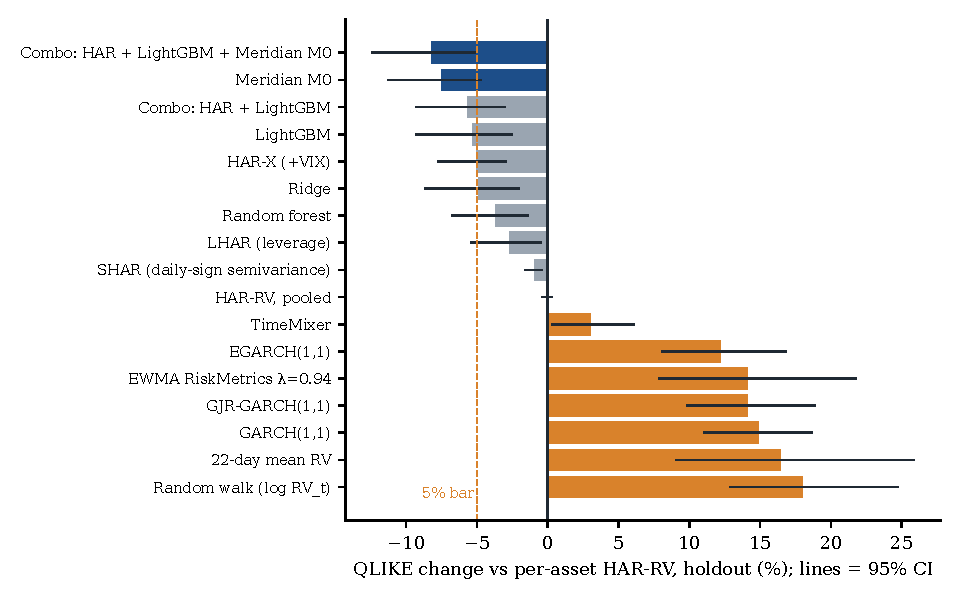
\includegraphics[width=0.92\linewidth]{generated/fig_vol_bars.pdf}
\caption{Holdout QLIKE change vs per-asset HAR-RV with 95\% block-bootstrap intervals. Blue: Meridian;
grey: better than HAR; orange: worse than HAR. Dashed line: the pre-registered 5\% bar.}\label{fig:volbars}
\end{figure}

\paragraph{Hit rate is not evidence of skill here.} Calibrated models' directional hit rates range only
from \HitMin\ to \HitMax: volatility is persistent, so predicting whether tomorrow's variance is above
today's is easy for any reasonable model. Hit rate is reported but not used to rank models.

\subsection{Conservative check against the strongest HAR}
On this holdout raw per-asset HAR (QLIKE \RawHARQ) scores better than its calibrated version
(\RawHARcalPct\ worse), so the most demanding comparison is against raw HAR (\cref{tab:volcons}).
Raw Meridian improves on it by \RawMPct\ \RawMCI, $p$ \RawMP; the combination by \RawComboPct\ \RawComboCI.

\begin{table}[!htbp]
\centering
\small
\caption{Conservative check: holdout against raw per-asset HAR, the strongest HAR form.}
\label{tab:volcons}
\begin{tabularx}{\linewidth}{X r l r r}
\toprule
\textbf{Model} & \textbf{QLIKE} & \textbf{vs raw HAR [95\% CI]} & \textbf{DM $p$} & \textbf{Won} \\
\midrule
\rowcolor{good}GR combo: HAR + LightGBM + Meridian M0 (pooled HAR anchor) & 0.3022 & $-7.0\%$ [-9.5, -4.9] & $<$0.001 & 11/11 \\
\rowcolor{good}Meridian M0 (pooled HAR anchor) --- raw & 0.3029 & $-6.8\%$ [-9.7, -4.5] & $<$0.001 & 11/11 \\
\rowcolor{good}Meridian M0 (pooled HAR anchor) --- calibrated & 0.3045 & $-6.3\%$ [-8.6, -4.3] & $<$0.001 & 11/11 \\
GR combo: HAR + LightGBM & 0.3105 & $-4.4\%$ [-6.6, -2.7] & $<$0.001 & 10/11 \\
LightGBM --- calibrated & 0.3118 & $-4.0\%$ [-6.5, -2.3] & $<$0.001 & 10/11 \\
HAR-RV, per asset --- raw & 0.3249 & $+0.0\%$  & --- & 0/11 \\
HAR-RV, per asset --- calibrated & 0.3292 & $+1.3\%$ [-0.2, +3.9] & 0.914 & 0/11 \\
\bottomrule
\end{tabularx}
\end{table}

\begin{table}[!htbp]
\centering
\scriptsize
\caption{Raw (uncalibrated) forecasts on the holdout, reference = raw per-asset HAR-RV.}
\label{tab:volraw}
\begin{tabularx}{\linewidth}{X l r l r r}
\toprule
\textbf{Model (raw, uncalibrated)} & \textbf{Family} & \textbf{QLIKE} & \textbf{vs raw HAR [95\% CI]} & \textbf{DM $p$} & \textbf{Won} \\
\midrule
\rowcolor{good}Meridian M0 (pooled HAR anchor) & Meridian & 0.3029 & $-6.8\%$ [-9.7, -4.5] & $<$0.001 & 11/11 \\
HAR-X (+VIX) & HAR & 0.3119 & $-4.0\%$ [-5.7, -2.5] & $<$0.001 & 10/11 \\
Ridge & ML & 0.3133 & $-3.6\%$ [-6.2, -1.3] & $<$0.001 & 10/11 \\
LightGBM & ML & 0.3137 & $-3.4\%$ [-6.3, -1.4] & 0.003 & 10/11 \\
LHAR (leverage) & HAR & 0.3159 & $-2.8\%$ [-4.8, -1.3] & 0.001 & 10/11 \\
Random forest & ML & 0.3195 & $-1.7\%$ [-4.0, +0.2] & 0.039 & 8/11 \\
SHAR (daily-sign semivariance) & HAR & 0.3218 & $-0.9\%$ [-1.6, -0.4] & 0.008 & 7/11 \\
HAR-RV, per asset (reference) & HAR & 0.3249 & $+0.0\%$  & --- & 0/11 \\
HAR-RV, pooled & HAR & 0.3285 & $+1.1\%$ [+0.4, +1.6] & 1.000 & 2/11 \\
TimeMixer & Deep & 0.3570 & $+9.9\%$ [+6.5, +13.9] & 1.000 & 0/11 \\
EWMA RiskMetrics $\lambda$=0.94 & Naive & 0.3627 & $+11.6\%$ [+6.2, +18.0] & 1.000 & 2/11 \\
22-day mean RV & Naive & 0.3779 & $+16.3\%$ [+10.6, +22.4] & 1.000 & 0/11 \\
EGARCH(1,1) & GARCH & 0.4218 & $+29.8\%$ [+25.1, +34.4] & 1.000 & 0/11 \\
GJR-GARCH(1,1) & GARCH & 0.4230 & $+30.2\%$ [+25.8, +34.2] & 1.000 & 0/11 \\
GARCH(1,1) & GARCH & 0.4307 & $+32.6\%$ [+28.2, +37.0] & 1.000 & 0/11 \\
Random walk (log RV\_t) & Naive & 0.5205 & $+60.2\%$ [+46.9, +69.5] & 1.000 & 0/11 \\
\bottomrule
\end{tabularx}
\end{table}


\subsection{Stability over time, assets and market conditions}
Meridian beats raw HAR in \YearsWon\ of \YearsTotal\ calendar years (\FirstYear--\LastYear; the
exception is \WorstYear, a partial year, at \WorstYearPct; \cref{fig:volyear,tab:volyear}). On the holdout
it beats HAR on every asset, from \AssetBestPct\ (\AssetBest) to \AssetWorstPct\ (\AssetWorst)
(\cref{fig:volasset,tab:volasset}). The gain is largest in high-VIX periods
(\RegStressPct\ in the stress tercile vs \RegCalmPct\ in the calm tercile; \cref{tab:volregime}).
On individual days the edge is noisy: Meridian has the lower loss on \ShareDay\ of holdout days, on
\ShareTwenty\ of 20-day windows, \ShareSixtyThree\ of 63-day windows and \ShareTwoFiftyTwo\ of
252-day windows (\cref{fig:volrolling}).

\begin{figure}[!htbp]
\centering
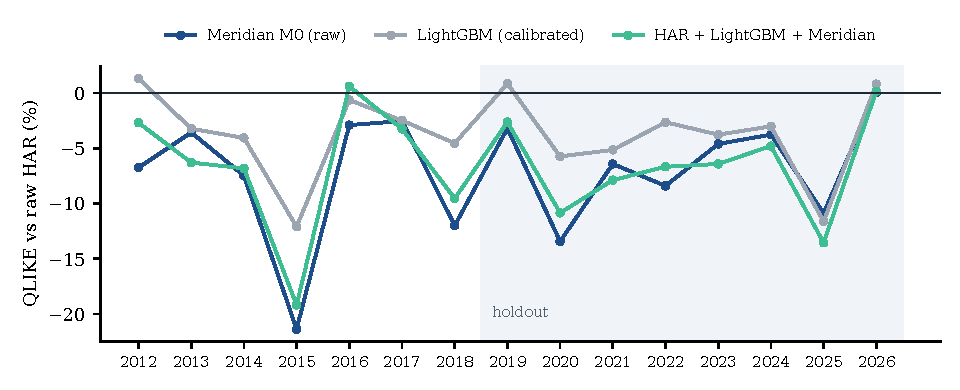
\includegraphics[width=0.92\linewidth]{generated/fig_vol_year.pdf}
\caption{QLIKE change vs raw per-asset HAR by calendar year (shaded: holdout).}\label{fig:volyear}
\end{figure}

\begin{figure}[!htbp]
\centering
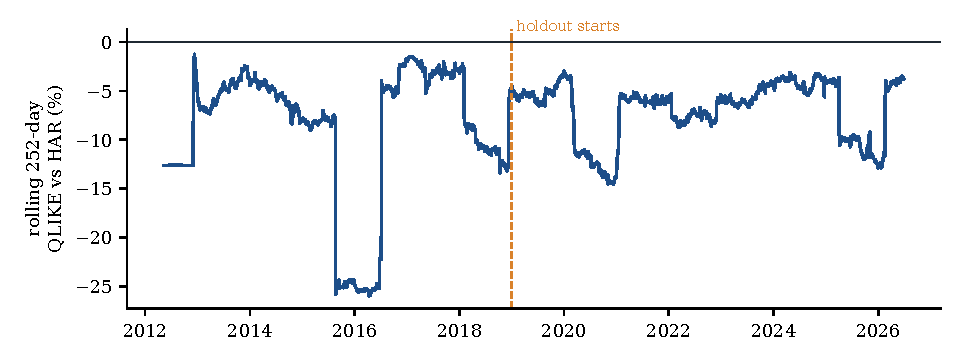
\includegraphics[width=0.92\linewidth]{generated/fig_vol_rolling.pdf}
\caption{Rolling 252-day QLIKE difference of raw Meridian vs raw per-asset HAR, as a percentage of HAR's
loss, over the full out-of-sample period.}\label{fig:volrolling}
\end{figure}

\begin{table}[!htbp]
\centering
\small
\caption{QLIKE change vs raw per-asset HAR by calendar year (all out-of-sample years).}
\label{tab:volyear}
\begin{tabularx}{\linewidth}{lrrrX}
\toprule
\textbf{Year} & \textbf{Meridian (raw)} & \textbf{LightGBM (cal.)} & \textbf{HAR+LGBM+Meridian} & \textbf{Period} \\
\midrule
2012 & $-6.7\%$ & $+1.3\%$ & $-2.7\%$ & development \\
2013 & $-3.6\%$ & $-3.2\%$ & $-6.3\%$ & development \\
2014 & $-7.5\%$ & $-4.1\%$ & $-6.8\%$ & development \\
2015 & $-21.4\%$ & $-12.1\%$ & $-19.2\%$ & development \\
2016 & $-2.9\%$ & $-0.6\%$ & $+0.6\%$ & development \\
2017 & $-2.5\%$ & $-2.5\%$ & $-3.2\%$ & development \\
2018 & $-12.0\%$ & $-4.5\%$ & $-9.5\%$ & development \\
2019 & $-3.2\%$ & $+0.8\%$ & $-2.6\%$ & holdout \\
2020 & $-13.4\%$ & $-5.7\%$ & $-10.8\%$ & holdout \\
2021 & $-6.4\%$ & $-5.1\%$ & $-7.9\%$ & holdout \\
2022 & $-8.4\%$ & $-2.6\%$ & $-6.7\%$ & holdout \\
2023 & $-4.6\%$ & $-3.8\%$ & $-6.4\%$ & holdout \\
2024 & $-3.8\%$ & $-3.0\%$ & $-4.8\%$ & holdout \\
2025 & $-10.9\%$ & $-11.6\%$ & $-13.5\%$ & holdout \\
2026 & $+0.0\%$ & $+0.8\%$ & $+0.2\%$ & holdout \\
\bottomrule
\end{tabularx}
\end{table}


\begin{figure}[!htbp]
\centering
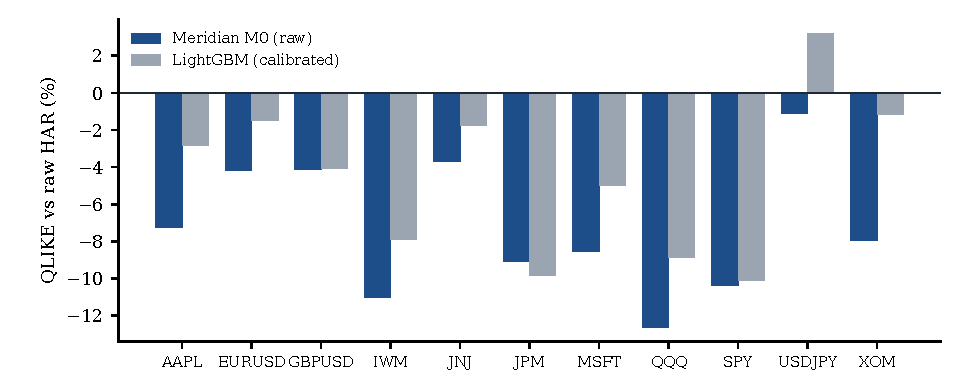
\includegraphics[width=0.92\linewidth]{generated/fig_vol_asset.pdf}
\caption{Holdout QLIKE change vs raw per-asset HAR, by asset.}\label{fig:volasset}
\end{figure}

\begin{table}[!htbp]
\centering
\small
\caption{Holdout QLIKE change vs raw per-asset HAR, by asset.}
\label{tab:volasset}
\begin{tabularx}{\linewidth}{Xrrrr}
\toprule
\textbf{Asset} & \textbf{Meridian (raw)} & \textbf{Meridian (cal.)} & \textbf{LightGBM (cal.)} & \textbf{HAR+LGBM+Meridian} \\
\midrule
AAPL & $-7.3\%$ & $-7.1\%$ & $-2.8\%$ & $-6.9\%$ \\
EURUSD & $-4.2\%$ & $-3.3\%$ & $-1.5\%$ & $-3.0\%$ \\
GBPUSD & $-4.1\%$ & $-1.3\%$ & $-4.1\%$ & $-4.1\%$ \\
IWM & $-11.0\%$ & $-10.6\%$ & $-7.9\%$ & $-10.1\%$ \\
JNJ & $-3.7\%$ & $-3.9\%$ & $-1.7\%$ & $-4.2\%$ \\
JPM & $-9.1\%$ & $-9.0\%$ & $-9.9\%$ & $-11.4\%$ \\
MSFT & $-8.5\%$ & $-8.4\%$ & $-5.0\%$ & $-8.3\%$ \\
QQQ & $-12.6\%$ & $-12.7\%$ & $-8.8\%$ & $-13.7\%$ \\
SPY & $-10.3\%$ & $-10.4\%$ & $-10.1\%$ & $-12.5\%$ \\
USDJPY & $-1.1\%$ & $-1.0\%$ & $+3.2\%$ & $-1.0\%$ \\
XOM & $-7.9\%$ & $-6.6\%$ & $-1.1\%$ & $-6.8\%$ \\
\bottomrule
\end{tabularx}
\end{table}

\begin{table}[!htbp]
\centering
\small
\caption{QLIKE change vs calibrated per-asset HAR by VIX tercile, full out-of-sample period (2012-08-13 to 2026-06-28); DM $p$ in brackets.}
\label{tab:volregime}
\begin{tabularx}{\linewidth}{Xlll}
\toprule
\textbf{Model} & \textbf{Calm} & \textbf{Normal} & \textbf{Stress} \\
\midrule
\rowcolor{good}Meridian M0 (pooled HAR anchor) & $-4.1\%$ ($<$0.001) & $-5.2\%$ ($<$0.001) & $-14.1\%$ (0.009) \\
\rowcolor{good}GR combo: HAR + LightGBM + Meridian M0 (pooled HAR anchor) & $-4.9\%$ ($<$0.001) & $-6.4\%$ (0.034) & $-15.3\%$ (0.005) \\
LightGBM & $-2.9\%$ ($<$0.001) & $-4.1\%$ (0.203) & $-10.9\%$ (0.004) \\
HAR-X (+VIX) & $-1.8\%$ ($<$0.001) & $-2.8\%$ ($<$0.001) & $-9.6\%$ (0.004) \\
Ridge & $-1.6\%$ ($<$0.001) & $-2.6\%$ ($<$0.001) & $-10.7\%$ (0.010) \\
LHAR (leverage) & $-1.2\%$ ($<$0.001) & $-2.2\%$ ($<$0.001) & $-7.1\%$ (0.035) \\
TimeMixer & $+2.6\%$ (0.975) & $+1.5\%$ (0.869) & $+3.3\%$ (0.931) \\
GJR-GARCH(1,1) & $+9.6\%$ (1.000) & $+8.1\%$ (1.000) & $+12.9\%$ (0.984) \\
EWMA RiskMetrics $\lambda$=0.94 & $+6.2\%$ (1.000) & $+9.0\%$ (1.000) & $+26.9\%$ (0.999) \\
\bottomrule
\end{tabularx}
\end{table}


\begin{figure}[!htbp]
\centering
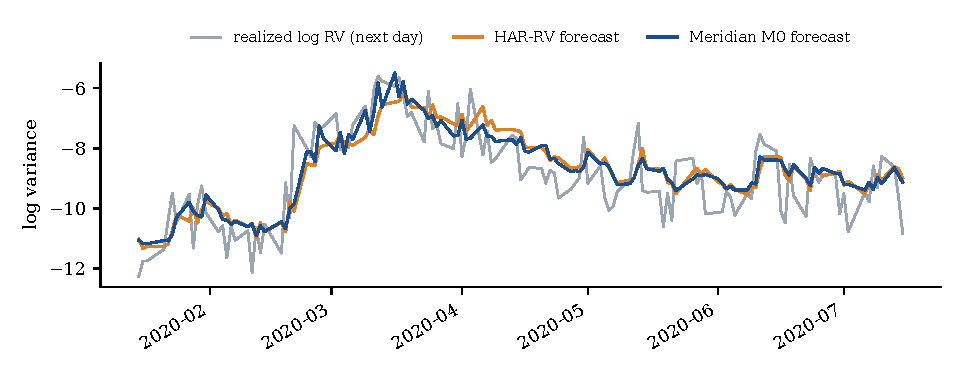
\includegraphics[width=0.92\linewidth]{generated/fig_vol_spy2020.pdf}
\caption{Illustration on real data: SPY, January--July 2020. Next-day realized log variance with the
HAR-RV and Meridian forecasts made the previous evening.}\label{fig:spy2020}
\end{figure}

\subsection{Longer horizons and out-of-universe assets}
At 5 days Meridian's auxiliary head improves on a horizon-specific HAR by \HFivePct\ ($p$ \HFiveP); at 22
days the difference, \HTwentyTwoPct, is not significant ($p$ \HTwentyTwoP) (\cref{tab:volhorizon}).
Only HAR and Meridian were compared at these horizons. On TLT and GLD, which the pooled models never
saw in training, calibrated Meridian improves on HAR by \BreadthMPct\ \BreadthMCI, $p$ \BreadthMP\
(\cref{tab:volbreadth}).

\begin{table}[!htbp]
\centering
\small
\caption{Longer horizons (holdout, calibrated): Meridian auxiliary heads vs per-asset HAR fit to the same horizon.}
\label{tab:volhorizon}
\begin{tabularx}{\linewidth}{Xrrlrr}
\toprule
\textbf{Horizon} & \textbf{HAR QLIKE} & \textbf{Meridian QLIKE} & \textbf{vs HAR [95\% CI]} & \textbf{DM $p$} & \textbf{Won} \\
\midrule
5 trading days & 0.1900 & 0.1718 & $-9.6\%$ [-14.5, -4.9] & $<$0.001 & 11/11 \\
22 trading days & 0.2086 & 0.2067 & $-0.9\%$ [-4.5, +6.7] & 0.356 & 7/11 \\
\bottomrule
\end{tabularx}
\end{table}

\begin{table}[!htbp]
\centering
\scriptsize
\caption{Out-of-universe check: TLT (long Treasuries) and GLD (gold), holdout. Pooled models (Meridian, Ridge, random forest, LightGBM, TimeMixer, pooled HAR) never trained on these assets.}
\label{tab:volbreadth}
\begin{tabularx}{\linewidth}{Xrlr}
\toprule
\textbf{Model (calibrated)} & \textbf{QLIKE} & \textbf{vs HAR [95\% CI]} & \textbf{DM $p$} \\
\midrule
\rowcolor{good}Meridian M0 (pooled HAR anchor) & 0.3086 & $-7.1\%$ [-12.4, -2.1] & 0.002 \\
HAR-X (+VIX) & 0.3265 & $-1.7\%$ [-6.6, +1.9] & 0.181 \\
HAR-RV, pooled & 0.3267 & $-1.6\%$ [-4.5, +1.1] & 0.110 \\
Ridge & 0.3300 & $-0.6\%$ [-7.0, +4.8] & 0.405 \\
HAR-RV, per asset (reference) & 0.3320 & $+0.0\%$  & --- \\
SHAR (daily-sign semivariance) & 0.3323 & $+0.1\%$ [-0.4, +0.8] & 0.613 \\
LHAR (leverage) & 0.3346 & $+0.8\%$ [-0.1, +1.8] & 0.931 \\
Random forest & 0.3377 & $+1.7\%$ [-2.1, +5.9] & 0.822 \\
LightGBM & 0.3473 & $+4.6\%$ [-0.4, +10.4] & 0.961 \\
EWMA RiskMetrics $\lambda$=0.94 & 0.3594 & $+8.2\%$ [+4.2, +12.8] & 1.000 \\
22-day mean RV & 0.3676 & $+10.7\%$ [+4.5, +17.7] & 1.000 \\
TimeMixer & 0.3716 & $+11.9\%$ [+6.5, +17.5] & 1.000 \\
GJR-GARCH(1,1) & 0.3861 & $+16.3\%$ [+6.4, +29.5] & 0.999 \\
EGARCH(1,1) & 0.3877 & $+16.8\%$ [+5.6, +32.2] & 0.995 \\
GARCH(1,1) & 0.3899 & $+17.4\%$ [+7.0, +31.2] & 0.999 \\
Random walk (log RV\_t) & 0.4001 & $+20.5\%$ [+11.4, +29.9] & 1.000 \\
\bottomrule
\end{tabularx}
\end{table}


\subsection{Development period and the improvement attempt}
Three architectural changes were proposed to improve Meridian and evaluated only on the development
period (\cref{tab:ablation,fig:ablation}): M1 replaces the pooled HAR anchor with a per-asset HAR
offset plus a zero-initialized correction; M2 adds a learned asset embedding; M3 adds early stopping.
None beat the existing configuration M0 (development QLIKE: M0 \AblMZero, M1 \AblMOne, M2 \AblMTwo,
M3 \AblMThree). This is recorded as a negative result; M0 was kept and the holdout was evaluated once.
\Cref{tab:voldev} gives the full development-period table of the final run (Meridian \DevMPct).

\begin{figure}[!htbp]
\centering
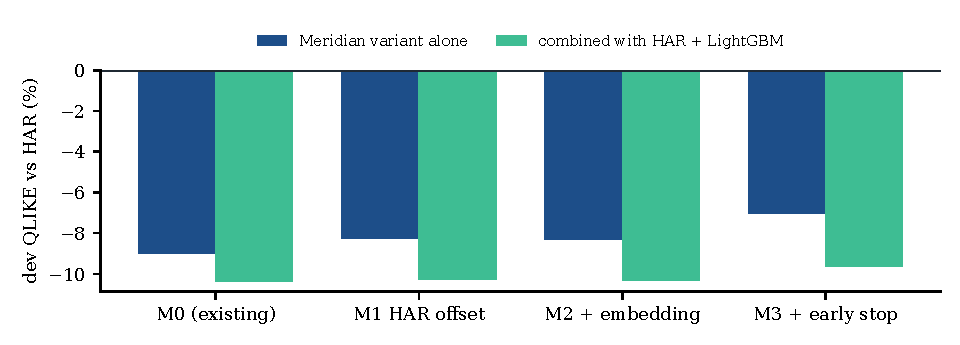
\includegraphics[width=0.85\linewidth]{generated/fig_ablation.pdf}
\caption{Development-period ablation: QLIKE change vs calibrated HAR for the existing configuration
(M0) and the three proposed changes, alone and in combination.}\label{fig:ablation}
\end{figure}

\begin{table}[!htbp]
\centering
\scriptsize
\caption{Development-period ablation of the proposed Meridian improvements (3 seeds each). The selection rule picks the lowest development QLIKE.}
\label{tab:ablation}
\begin{tabularx}{\linewidth}{XXrr}
\toprule
\textbf{Candidate} & \textbf{Change tested} & \textbf{Dev QLIKE} & \textbf{vs HAR} \\
\midrule
\rowcolor{good}GR combo: HAR + LightGBM + Meridian M0 (pooled HAR anchor) & pooled HAR-anchored initialization (existing) & 0.3353 & $-10.4\%$ \\
GR combo: HAR + LightGBM + Meridian M2 (M1 + asset embedding) & M1 + learned asset embedding & 0.3354 & $-10.3\%$ \\
GR combo: HAR + LightGBM + Meridian M1 (per-asset HAR offset) & per-asset HAR offset + zero-init correction & 0.3356 & $-10.3\%$ \\
GR combo: HAR + LightGBM + Meridian M3 (M1 + early stopping) & M1 + early stopping (purged validation slice) & 0.3381 & $-9.6\%$ \\
Meridian M0 (pooled HAR anchor) & pooled HAR-anchored initialization (existing) & 0.3404 & $-9.0\%$ \\
Meridian M2 (M1 + asset embedding) & M1 + learned asset embedding & 0.3430 & $-8.3\%$ \\
Meridian M1 (per-asset HAR offset) & per-asset HAR offset + zero-init correction & 0.3432 & $-8.3\%$ \\
Meridian M3 (M1 + early stopping) & M1 + early stopping (purged validation slice) & 0.3477 & $-7.1\%$ \\
HAR-RV, per asset (reference) & reference & 0.3741 & $+0.0\%$ \\
\bottomrule
\end{tabularx}
\end{table}

\begin{table}[!htbp]
\centering
\scriptsize
\caption{Development period 2012-06-14 to 2018-12-31 (final 5-seed run).}
\label{tab:voldev}
\begin{tabularx}{\linewidth}{Xrlrr}
\toprule
\textbf{Model (calibrated)} & \textbf{QLIKE} & \textbf{vs HAR [95\% CI]} & \textbf{DM $p$} & \textbf{Won} \\
\midrule
\rowcolor{good}GR combo: HAR + LightGBM + Meridian M0 (pooled HAR anchor) & 0.3356 & $-10.3\%$ [-16.3, -5.4] & 0.017 & 11/11 \\
\rowcolor{good}Meridian M0 (pooled HAR anchor) & 0.3410 & $-8.8\%$ [-15.2, -3.8] & 0.016 & 11/11 \\
GR combo: HAR + LightGBM & 0.3461 & $-7.5\%$ [-11.2, -4.1] & 0.034 & 11/11 \\
LightGBM & 0.3469 & $-7.3\%$ [-10.9, -4.0] & 0.023 & 10/11 \\
Random forest & 0.3515 & $-6.0\%$ [-9.7, -3.1] & 0.042 & 10/11 \\
Ridge & 0.3528 & $-5.7\%$ [-10.4, -2.3] & 0.038 & 10/11 \\
HAR-X (+VIX) & 0.3552 & $-5.0\%$ [-8.6, -2.3] & 0.025 & 11/11 \\
LHAR (leverage) & 0.3561 & $-4.8\%$ [-9.0, -1.6] & 0.040 & 11/11 \\
SHAR (daily-sign semivariance) & 0.3696 & $-1.2\%$ [-2.6, -0.0] & 0.061 & 9/11 \\
HAR-RV, pooled & 0.3728 & $-0.3\%$ [-0.6, -0.1] & 0.011 & 7/11 \\
HAR-RV, per asset (reference) & 0.3741 & $+0.0\%$  & --- & 0/11 \\
TimeMixer & 0.3818 & $+2.1\%$ [-0.2, +4.3] & 0.966 & 3/11 \\
GJR-GARCH(1,1) & 0.3987 & $+6.6\%$ [-0.4, +12.0] & 0.958 & 4/11 \\
EGARCH(1,1) & 0.4004 & $+7.0\%$ [+1.9, +11.4] & 0.996 & 2/11 \\
Random walk (log RV\_t) & 0.4028 & $+7.7\%$ [+0.0, +13.6] & 0.993 & 1/11 \\
GARCH(1,1) & 0.4218 & $+12.8\%$ [+8.9, +16.1] & 1.000 & 0/11 \\
EWMA RiskMetrics $\lambda$=0.94 & 0.4319 & $+15.5\%$ [+8.5, +23.7] & 0.995 & 1/11 \\
22-day mean RV & 0.4349 & $+16.3\%$ [+9.3, +24.3] & 0.996 & 0/11 \\
\bottomrule
\end{tabularx}
\end{table}


% ================================================================== 9
\section{Results: tail risk (Value-at-Risk and Expected Shortfall)}\label{sec:tail}

\subsection{Question and models}
Does Meridian's volatility forecast produce better next-day VaR and ES of close-to-close returns than the
standard risk models? Levels $\alpha\in\{1\%, 2.5\%, 5\%\}$; zero conditional mean for all models;
same folds as \cref{sec:vol}. The design (Amendment 7) was declared before any result was computed.

\begin{table}[!htbp]
\centering\small
\caption{Tail-risk models compared.}\label{tab:tailmodels}
\begin{tabularx}{\linewidth}{l X}
\toprule
\textbf{Model} & \textbf{Specification} \\
\midrule
Historical simulation & empirical quantile and tail mean of the last \TailHS\ returns \\
RiskMetrics & EWMA variance ($\lambda=0.94$), normal \\
GARCH(1,1)-normal / -$t$ & parametric VaR/ES \\
GJR-GARCH-skewed-$t$ & Hansen skewed-$t$ \cite{hansen1994} \\
GJR-GARCH + FHS (reference) & filtered historical simulation \cite{baroneadesi1999} \\
GJR-GARCH + EVT & GPD on standardized residuals \cite{mcneilfrey2000} \\
CAViaR (asymmetric slope) & quantile autoregression \cite{englemanganelli2004}; VaR only \\
HAR / LightGBM / Meridian + FHS & returns filtered by the saved out-of-sample volatility forecast \\
HAR / Meridian + EVT & as above with a GPD tail \\
Meridian + FHS + ACI & adaptive conformal level \cite{gibbscandes2021}, $\gamma=\TailGamma$ \\
\bottomrule
\end{tabularx}
\end{table}

\begin{algorithm}[!htbp]
\caption{Volatility-filtered VaR/ES (FHS and EVT variants), forecast at origin $t$}\label{alg:tail}
\begin{algorithmic}[1]
\Require volatility forecasts $\hat\sigma_{s+1\mid s}$ and returns $r_{s+1}$ for origins $s<t$
\State $z_s \gets r_{s+1}/\hat\sigma_{s+1\mid s}$ for the last $\le\TailZWin$ origins $s<t$ (need $\ge\TailZMin$)
\If{FHS}
  \State $q_\alpha \gets$ empirical $\alpha$-quantile of $z$; \ $e_\alpha \gets$ mean of $z$ below $q_\alpha$
\Else \Comment{EVT, refit every \TailRefit\ days}
  \State $u \gets$ \TailEVTu-quantile of losses $-z$; fit GPD$(\xi,\beta)$ to exceedances over $u$
  \State $q_\alpha \gets -\bigl[u + \tfrac{\beta}{\xi}\bigl((\tfrac{n\alpha}{N_u})^{-\xi}-1\bigr)\bigr]$;
         \ $e_\alpha \gets -\tfrac{-q_\alpha + \beta - \xi u}{1-\xi}$
\EndIf
\State \Return $\mathrm{VaR}_t = \hat\sigma_{t+1\mid t}\,q_\alpha$, \ $\mathrm{ES}_t = \hat\sigma_{t+1\mid t}\,e_\alpha$
\end{algorithmic}
\end{algorithm}

\paragraph{Scoring.} The primary score is the FZ0 loss \cite{fisslerziegel2016,pattonziegelchen2019},
which is strictly consistent for the pair (VaR, ES):
\begin{equation}
L_{\text{FZ0}}(v,e;r) = -\frac{1}{\alpha e}\,\mathbf{1}\{r\le v\}(v-r) + \frac{v}{e} + \ln(-e) - 1,
\qquad e\le v<0 .
\end{equation}
Differences in FZ0 between models are invariant to each asset's return scale, so assets can be pooled.
VaR alone is scored by the quantile loss $(\alpha - \mathbf{1}\{r<v\})(r-v)$ on returns divided by a
fixed per-asset scale. Absolute calibration is checked per asset with the Kupiec unconditional-coverage
test \cite{kupiec1995}, the Christoffersen conditional-coverage test \cite{christoffersen1998} and the
Engle--Manganelli dynamic-quantile (DQ) test; ES with the realized/forecast ratio on violation days.
Comparative significance uses the same date-level DM test, bootstrap and MCS as \cref{sec:protocol}.
The Meridian variant (FHS, EVT or FHS+ACI) was chosen on the development period: \TailSel.

\subsection{Results}
\TailSel\ has the lowest joint VaR+ES loss on the holdout: FZ0 difference \TFZ\ \TFZCI\ vs the GJR-GARCH
+ FHS reference, $p$ \TFZP\ (\cref{tab:tailfz,fig:tailfz}). Its violation rates are \TViolOne, \TViolTwo\
and \TViolFive\ at the 1\%, 2.5\% and 5\% levels; it passes the Kupiec and Christoffersen tests on
\TKupOne/11 and \TCCOne/11 assets at 1\% and \TKupFive/11 and \TCCFive/11 at 5\%, and the DQ test on
\TDQ/11 assets at 2.5\%; realized tail losses are \TESR\ times the forecast ES. At 1\% its quantile loss is
\TVOne\ \TVOneCI\ vs the reference ($p$ \TVOneP). Historical simulation is worst (\THSOne\ at 1\%), and
the normal-based models under-cover at 1\% (violation rates \TGNOneViol\ for GARCH-normal and
\TRMOneViol\ for RiskMetrics).

\begin{table}[!htbp]
\centering
\scriptsize
\caption{Joint VaR + ES at 2.5\% (FZ0 loss, lower is better), holdout 2019-01-01 to 2026-06-29 (2,168 dates $\times$ 11 assets). Reference: GJR-GARCH + filtered historical simulation.}
\label{tab:tailfz}
\begin{tabularx}{\linewidth}{>{\raggedright\arraybackslash}X r l r c r l r}
\toprule
\textbf{Model} & \textbf{FZ0} & \textbf{$\Delta$ vs reference [95\% CI]} & \textbf{DM $p$} & \textbf{MCS} & \textbf{Viol.\ \%} & \textbf{CC $\cdot$ DQ pass} & \textbf{ES ratio} \\
\midrule
\rowcolor{good}Meridian + FHS & -3.6394 & -0.1226 [-0.1530, -0.0959] & $<$0.001 & \checkmark & 2.54 & 11/11 $\cdot$ 10/11 & 0.97 \\
\rowcolor{good}Meridian + EVT & -3.6387 & -0.1218 [-0.1533, -0.0949] & $<$0.001 & \checkmark & 2.49 & 11/11 $\cdot$ 10/11 & 0.98 \\
HAR-RV + FHS & -3.6289 & -0.1182 [-0.1440, -0.0927] & $<$0.001 & \checkmark & 2.58 & 11/11 $\cdot$ 8/11 & 0.99 \\
HAR-RV + EVT & -3.6284 & -0.1179 [-0.1449, -0.0912] & $<$0.001 & \checkmark & 2.57 & 11/11 $\cdot$ 7/11 & 0.99 \\
\rowcolor{good}Meridian + FHS + adaptive conformal & -3.6257 & -0.1080 [-0.1448, -0.0782] & $<$0.001 &  & 2.47 & 11/11 $\cdot$ 11/11 & 0.98 \\
LightGBM vol + FHS & -3.6208 & -0.1048 [-0.1306, -0.0796] & $<$0.001 &  & 2.58 & 11/11 $\cdot$ 10/11 & 0.98 \\
GJR-GARCH-skewed-t & -3.5294 & -0.0013 [-0.0124, +0.0093] & 0.404 &  & 2.60 & 10/11 $\cdot$ 10/11 & 0.99 \\
GJR-GARCH + EVT (McNeil-Frey) & -3.5290 & -0.0030 [-0.0054, -0.0007] & 0.007 &  & 2.67 & 11/11 $\cdot$ 11/11 & 0.98 \\
GJR-GARCH + FHS (reference) & -3.5255 & --- & --- &  & 2.71 & 11/11 $\cdot$ 11/11 & 0.98 \\
\rowcolor{bad}GARCH(1,1)-t & -3.5203 & +0.0067 [-0.0097, +0.0234] & 0.799 &  & 2.87 & 10/11 $\cdot$ 7/11 & 1.00 \\
\rowcolor{bad}GARCH(1,1)-normal & -3.5049 & +0.0179 [-0.0036, +0.0427] & 0.951 &  & 3.01 & 9/11 $\cdot$ 7/11 & 1.14 \\
\rowcolor{bad}RiskMetrics EWMA, normal & -3.4538 & +0.0626 [+0.0215, +0.1094] & 0.999 &  & 3.48 & 4/11 $\cdot$ 1/11 & 1.16 \\
\rowcolor{bad}Historical simulation (500d) & -3.3320 & +0.1836 [+0.0660, +0.3735] & 0.997 &  & 2.80 & 5/11 $\cdot$ 1/11 & 1.07 \\
\bottomrule
\end{tabularx}
\end{table}


\begin{figure}[!htbp]
\centering
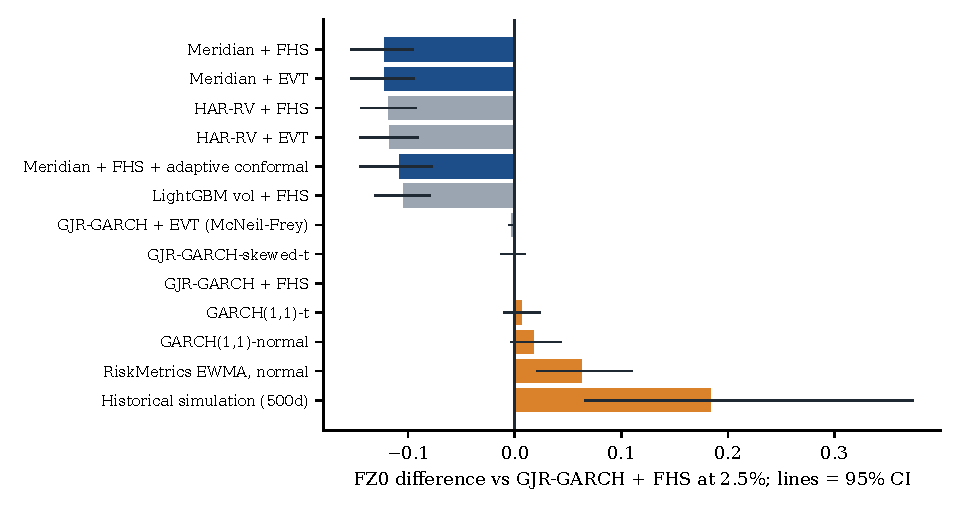
\includegraphics[width=0.92\linewidth]{generated/fig_tail_fz.pdf}
\caption{Holdout FZ0 loss difference vs GJR-GARCH + FHS at 2.5\%, with 95\% intervals.}\label{fig:tailfz}
\end{figure}

\begin{keybox}[The honest reading of the tail results]
The clear separation is between models that use a range-based realized-volatility forecast (Meridian,
HAR, LightGBM) and models that use returns only (GARCH family, RiskMetrics, historical simulation,
CAViaR). Against the HAR-filtered tail the Meridian advantage is \textbf{not statistically significant}
(\cref{tab:tailh2h}: $p$ \HHOneP\ at 1\%, \HHTwoP\ at 2.5\%, \HHFiveP\ at 5\%). On the development period
the HAR-filtered tail was in fact slightly better (FZ0 \TDevHAR\ vs \TDevSel; \cref{tab:taildev}).
Meridian's tails do cluster less: they pass the DQ test on \TDQ/11 assets vs \THarDQ/11 for HAR + FHS.
\end{keybox}

\begin{table}[!htbp]
\centering
\small
\caption{Head-to-head on the holdout: Meridian + EVT vs HAR-RV + FHS (both filtered by a realized-volatility forecast).}
\label{tab:tailh2h}
\begin{tabularx}{\linewidth}{lXrXr}
\toprule
\textbf{Level} & \textbf{FZ0 $\Delta$ [95\% CI]} & \textbf{DM $p$} & \textbf{Quantile loss vs HAR-FHS [95\% CI]} & \textbf{DM $p$} \\
\midrule
1\% & -0.0100 [-0.0461, +0.0168] & 0.245 & $-3.1\%$ [-7.4, +0.2] & 0.076 \\
2.5\% & -0.0037 [-0.0333, +0.0175] & 0.369 & $-2.0\%$ [-6.2, +1.1] & 0.159 \\
5\% & -0.0013 [-0.0246, +0.0144] & 0.439 & $-1.1\%$ [-4.1, +1.0] & 0.203 \\
\bottomrule
\end{tabularx}
\end{table}


\begin{figure}[!htbp]
\centering
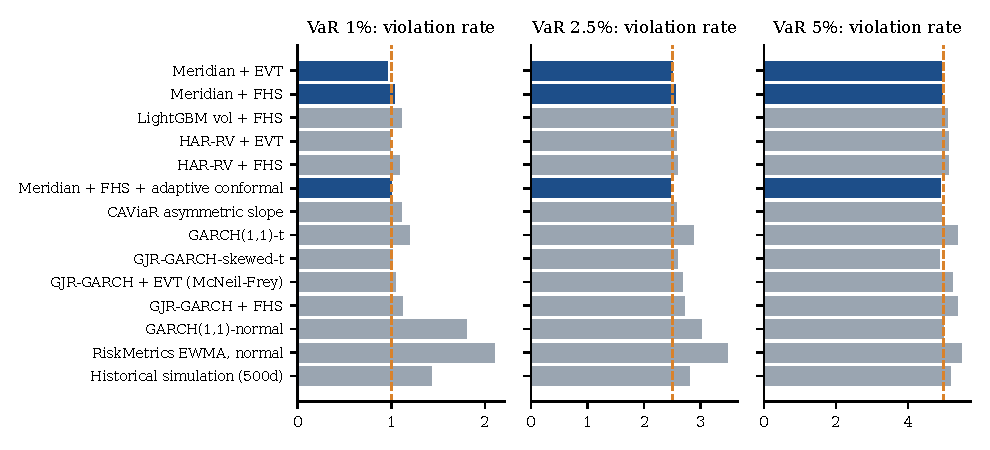
\includegraphics[width=0.95\linewidth]{generated/fig_tail_viol.pdf}
\caption{Holdout VaR violation rates by model; dashed lines mark the nominal level.}\label{fig:tailviol}
\end{figure}

\begin{table}[!htbp]
\centering
\scriptsize
\caption{VaR at 1\%: quantile loss on returns scaled per asset, holdout.}
\label{tab:tailvar010}
\begin{tabularx}{\linewidth}{>{\raggedright\arraybackslash}X r l r c r l}
\toprule
\textbf{Model} & \textbf{Loss $\times10^3$} & \textbf{vs reference [95\% CI]} & \textbf{DM $p$} & \textbf{MCS} & \textbf{Viol.\ \% (target 1)} & \textbf{Kupiec $\cdot$ CC $\cdot$ DQ pass (of 11)} \\
\midrule
\rowcolor{good}Meridian + EVT & 22.27 & $-9.2\%$ [-12.7, -5.9] & $<$0.001 & \checkmark & 0.96 & 11 $\cdot$ 11 $\cdot$ 10 \\
\rowcolor{good}Meridian + FHS & 22.32 & $-9.0\%$ [-12.5, -5.7] & $<$0.001 & \checkmark & 1.04 & 11 $\cdot$ 11 $\cdot$ 10 \\
LightGBM vol + FHS & 22.59 & $-7.9\%$ [-10.8, -4.7] & $<$0.001 & \checkmark & 1.11 & 11 $\cdot$ 11 $\cdot$ 10 \\
HAR-RV + EVT & 22.98 & $-6.3\%$ [-9.7, -2.5] & $<$0.001 & \checkmark & 0.99 & 11 $\cdot$ 10 $\cdot$ 7 \\
HAR-RV + FHS & 22.99 & $-6.3\%$ [-9.6, -2.7] & $<$0.001 & \checkmark & 1.09 & 11 $\cdot$ 10 $\cdot$ 6 \\
\rowcolor{good}Meridian + FHS + adaptive conformal & 23.26 & $-5.2\%$ [-9.1, -1.5] & $<$0.001 &  & 1.00 & 11 $\cdot$ 11 $\cdot$ 11 \\
CAViaR asymmetric slope & 24.21 & $-1.3\%$ [-2.9, +0.6] & 0.181 &  & 1.11 & 10 $\cdot$ 10 $\cdot$ 10 \\
GARCH(1,1)-t & 24.39 & $-0.6\%$ [-2.7, +1.7] & 0.357 &  & 1.19 & 9 $\cdot$ 11 $\cdot$ 8 \\
GJR-GARCH-skewed-t & 24.47 & $-0.3\%$ [-1.4, +1.1] & 0.437 &  & 1.01 & 11 $\cdot$ 11 $\cdot$ 11 \\
GJR-GARCH + EVT (McNeil-Frey) & 24.51 & $-0.1\%$ [-0.5, +0.4] & 0.411 &  & 1.05 & 11 $\cdot$ 11 $\cdot$ 11 \\
GJR-GARCH + FHS (reference) & 24.53 & $+0.0\%$  & --- &  & 1.12 & 11 $\cdot$ 11 $\cdot$ 10 \\
GARCH(1,1)-normal & 25.08 & $+2.2\%$ [-1.9, +7.3] & 0.828 &  & 1.80 & 2 $\cdot$ 2 $\cdot$ 2 \\
RiskMetrics EWMA, normal & 26.37 & $+7.5\%$ [+0.1, +17.1] & 0.972 &  & 2.10 & 0 $\cdot$ 0 $\cdot$ 0 \\
Historical simulation (500d) & 30.97 & $+26.3\%$ [+6.7, +57.4] & 0.980 &  & 1.43 & 8 $\cdot$ 4 $\cdot$ 0 \\
\bottomrule
\end{tabularx}
\end{table}

\begin{table}[!htbp]
\centering
\scriptsize
\caption{VaR at 2.5\%: quantile loss on returns scaled per asset, holdout.}
\label{tab:tailvar025}
\begin{tabularx}{\linewidth}{>{\raggedright\arraybackslash}X r l r c r l}
\toprule
\textbf{Model} & \textbf{Loss $\times10^3$} & \textbf{vs reference [95\% CI]} & \textbf{DM $p$} & \textbf{MCS} & \textbf{Viol.\ \% (target 2.5)} & \textbf{Kupiec $\cdot$ CC $\cdot$ DQ pass (of 11)} \\
\midrule
\rowcolor{good}Meridian + FHS & 45.54 & $-7.4\%$ [-9.6, -5.2] & $<$0.001 & \checkmark & 2.54 & 11 $\cdot$ 11 $\cdot$ 10 \\
\rowcolor{good}Meridian + EVT & 45.54 & $-7.4\%$ [-9.7, -5.1] & $<$0.001 & \checkmark & 2.49 & 11 $\cdot$ 11 $\cdot$ 10 \\
LightGBM vol + FHS & 46.10 & $-6.3\%$ [-8.4, -4.0] & $<$0.001 &  & 2.58 & 11 $\cdot$ 11 $\cdot$ 10 \\
\rowcolor{good}Meridian + FHS + adaptive conformal & 46.11 & $-6.2\%$ [-9.4, -3.5] & $<$0.001 &  & 2.47 & 11 $\cdot$ 11 $\cdot$ 11 \\
HAR-RV + FHS & 46.46 & $-5.5\%$ [-8.0, -2.7] & $<$0.001 & \checkmark & 2.58 & 11 $\cdot$ 11 $\cdot$ 8 \\
HAR-RV + EVT & 46.56 & $-5.3\%$ [-8.1, -2.2] & $<$0.001 & \checkmark & 2.57 & 11 $\cdot$ 11 $\cdot$ 7 \\
GJR-GARCH-skewed-t & 48.89 & $-0.6\%$ [-2.3, +0.7] & 0.231 &  & 2.60 & 10 $\cdot$ 10 $\cdot$ 10 \\
GJR-GARCH + EVT (McNeil-Frey) & 49.04 & $-0.3\%$ [-0.5, -0.1] & 0.005 &  & 2.67 & 11 $\cdot$ 11 $\cdot$ 11 \\
CAViaR asymmetric slope & 49.09 & $-0.2\%$ [-1.6, +1.3] & 0.730 &  & 2.57 & 8 $\cdot$ 9 $\cdot$ 9 \\
GJR-GARCH + FHS (reference) & 49.18 & $+0.0\%$  & --- &  & 2.71 & 11 $\cdot$ 11 $\cdot$ 11 \\
GARCH(1,1)-normal & 49.36 & $+0.4\%$ [-1.0, +2.1] & 0.684 &  & 3.01 & 6 $\cdot$ 9 $\cdot$ 7 \\
GARCH(1,1)-t & 49.41 & $+0.5\%$ [-0.8, +1.9] & 0.780 &  & 2.87 & 8 $\cdot$ 10 $\cdot$ 7 \\
RiskMetrics EWMA, normal & 50.84 & $+3.4\%$ [+0.4, +7.2] & 0.979 &  & 3.48 & 3 $\cdot$ 4 $\cdot$ 1 \\
Historical simulation (500d) & 56.55 & $+15.0\%$ [+3.9, +31.6] & 0.987 &  & 2.80 & 11 $\cdot$ 5 $\cdot$ 1 \\
\bottomrule
\end{tabularx}
\end{table}

\begin{table}[!htbp]
\centering
\scriptsize
\caption{VaR at 5\%: quantile loss on returns scaled per asset, holdout.}
\label{tab:tailvar050}
\begin{tabularx}{\linewidth}{>{\raggedright\arraybackslash}X r l r c r l}
\toprule
\textbf{Model} & \textbf{Loss $\times10^3$} & \textbf{vs reference [95\% CI]} & \textbf{DM $p$} & \textbf{MCS} & \textbf{Viol.\ \% (target 5)} & \textbf{Kupiec $\cdot$ CC $\cdot$ DQ pass (of 11)} \\
\midrule
\rowcolor{good}Meridian + EVT & 77.07 & $-5.1\%$ [-6.7, -3.6] & $<$0.001 & \checkmark & 4.95 & 11 $\cdot$ 11 $\cdot$ 9 \\
\rowcolor{good}Meridian + FHS & 77.17 & $-5.0\%$ [-6.5, -3.5] & $<$0.001 &  & 4.97 & 11 $\cdot$ 11 $\cdot$ 9 \\
\rowcolor{good}Meridian + FHS + adaptive conformal & 77.74 & $-4.3\%$ [-6.2, -2.5] & $<$0.001 &  & 4.90 & 11 $\cdot$ 11 $\cdot$ 9 \\
LightGBM vol + FHS & 77.78 & $-4.2\%$ [-5.6, -2.9] & $<$0.001 &  & 5.11 & 11 $\cdot$ 11 $\cdot$ 9 \\
HAR-RV + FHS & 77.94 & $-4.0\%$ [-5.7, -2.1] & $<$0.001 & \checkmark & 5.13 & 11 $\cdot$ 11 $\cdot$ 8 \\
HAR-RV + EVT & 77.95 & $-4.0\%$ [-5.7, -2.1] & $<$0.001 & \checkmark & 5.12 & 11 $\cdot$ 11 $\cdot$ 7 \\
GJR-GARCH-skewed-t & 80.79 & $-0.5\%$ [-2.0, +0.6] & 0.222 &  & 4.89 & 9 $\cdot$ 10 $\cdot$ 10 \\
GJR-GARCH + EVT (McNeil-Frey) & 81.12 & $-0.1\%$ [-0.2, -0.0] & 0.063 &  & 5.25 & 11 $\cdot$ 10 $\cdot$ 10 \\
CAViaR asymmetric slope & 81.21 & $-0.0\%$ [-1.2, +1.0] & 0.788 &  & 4.95 & 8 $\cdot$ 8 $\cdot$ 9 \\
GJR-GARCH + FHS (reference) & 81.22 & $+0.0\%$  & --- &  & 5.37 & 11 $\cdot$ 10 $\cdot$ 9 \\
GARCH(1,1)-normal & 81.57 & $+0.4\%$ [-0.5, +1.4] & 0.925 &  & 4.99 & 8 $\cdot$ 10 $\cdot$ 9 \\
GARCH(1,1)-t & 81.83 & $+0.7\%$ [-0.0, +1.6] & 0.969 &  & 5.37 & 8 $\cdot$ 10 $\cdot$ 7 \\
RiskMetrics EWMA, normal & 83.19 & $+2.4\%$ [+0.8, +4.0] & 0.999 &  & 5.48 & 10 $\cdot$ 10 $\cdot$ 3 \\
Historical simulation (500d) & 89.55 & $+10.3\%$ [+3.4, +20.1] & 0.996 &  & 5.17 & 11 $\cdot$ 5 $\cdot$ 1 \\
\bottomrule
\end{tabularx}
\end{table}


\begin{figure}[!htbp]
\centering
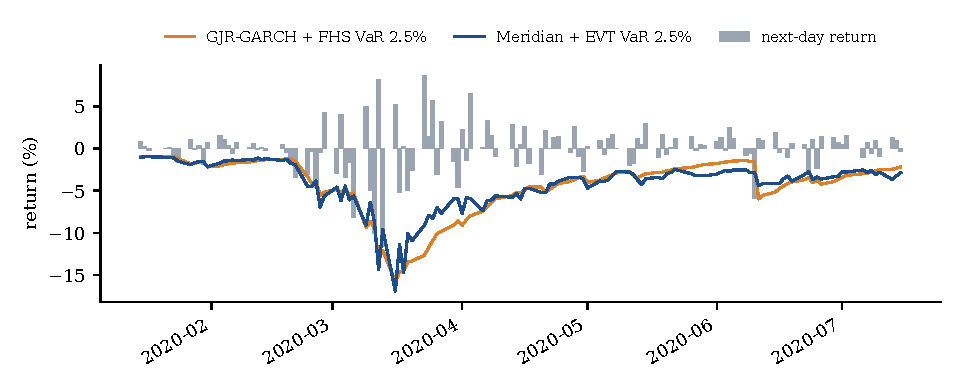
\includegraphics[width=0.92\linewidth]{generated/fig_tail_spy2020.pdf}
\caption{Illustration on real data: SPY next-day returns and 2.5\% VaR forecasts, January--July 2020.}
\label{fig:tailspy}
\end{figure}

\begin{table}[!htbp]
\centering
\scriptsize
\caption{Tail benchmark, development period (used only to choose the Meridian tail variant), 2.5\%.}
\label{tab:taildev}
\begin{tabularx}{\linewidth}{>{\raggedright\arraybackslash}X r l r c r l r}
\toprule
\textbf{Model} & \textbf{FZ0} & \textbf{$\Delta$ vs reference [95\% CI]} & \textbf{DM $p$} & \textbf{MCS} & \textbf{Viol.\ \%} & \textbf{CC $\cdot$ DQ pass} & \textbf{ES ratio} \\
\midrule
HAR-RV + FHS & -3.7832 & -0.0998 [-0.1247, -0.0724] & $<$0.001 & \checkmark & 2.61 & 10/11 $\cdot$ 7/11 & 1.04 \\
HAR-RV + EVT & -3.7830 & -0.0981 [-0.1230, -0.0710] & $<$0.001 & \checkmark & 2.46 & 9/11 $\cdot$ 8/11 & 1.04 \\
\rowcolor{good}Meridian + EVT & -3.7753 & -0.0865 [-0.1159, -0.0585] & $<$0.001 & \checkmark & 2.47 & 10/11 $\cdot$ 9/11 & 1.04 \\
\rowcolor{good}Meridian + FHS & -3.7746 & -0.0862 [-0.1164, -0.0573] & $<$0.001 & \checkmark & 2.63 & 10/11 $\cdot$ 8/11 & 1.03 \\
\rowcolor{good}Meridian + FHS + adaptive conformal & -3.7547 & -0.0677 [-0.0976, -0.0393] & $<$0.001 &  & 2.53 & 10/11 $\cdot$ 9/11 & 1.04 \\
LightGBM vol + FHS & -3.7514 & -0.0595 [-0.0850, -0.0327] & $<$0.001 &  & 2.68 & 11/11 $\cdot$ 9/11 & 1.03 \\
GJR-GARCH + EVT (McNeil-Frey) & -3.7034 & -0.0002 [-0.0027, +0.0024] & 0.452 &  & 2.23 & 9/11 $\cdot$ 9/11 & 1.05 \\
GJR-GARCH + FHS (reference) & -3.7016 & --- & --- &  & 2.33 & 9/11 $\cdot$ 9/11 & 1.03 \\
\rowcolor{bad}GJR-GARCH-skewed-t & -3.6911 & +0.0161 [-0.0003, +0.0293] & 0.983 &  & 1.88 & 5/11 $\cdot$ 8/11 & 1.05 \\
\rowcolor{bad}GARCH(1,1)-t & -3.6842 & +0.0204 [+0.0087, +0.0329] & 0.999 &  & 2.21 & 8/11 $\cdot$ 10/11 & 1.06 \\
\rowcolor{bad}GARCH(1,1)-normal & -3.6804 & +0.0187 [+0.0036, +0.0379] & 0.980 &  & 2.33 & 10/11 $\cdot$ 9/11 & 1.18 \\
\rowcolor{bad}RiskMetrics EWMA, normal & -3.6207 & +0.0676 [+0.0230, +0.1249] & 0.995 &  & 3.26 & 5/11 $\cdot$ 3/11 & 1.21 \\
\rowcolor{bad}Historical simulation (500d) & -3.5578 & +0.1409 [+0.0936, +0.1979] & 1.000 &  & 2.84 & 4/11 $\cdot$ 0/11 & 1.04 \\
\bottomrule
\end{tabularx}
\end{table}

\begin{table}[!htbp]
\centering
\scriptsize
\caption{Tail benchmark on the out-of-universe assets TLT and GLD, holdout, 2.5\%.}
\label{tab:tailbreadth}
\begin{tabularx}{\linewidth}{>{\raggedright\arraybackslash}X r l r c r l r}
\toprule
\textbf{Model} & \textbf{FZ0} & \textbf{$\Delta$ vs reference [95\% CI]} & \textbf{DM $p$} & \textbf{MCS} & \textbf{Viol.\ \%} & \textbf{CC $\cdot$ DQ pass} & \textbf{ES ratio} \\
\midrule
\rowcolor{good}Meridian + EVT & -3.7059 & -0.0638 [-0.1344, -0.0057] & 0.015 &  & 2.71 & 2/2 $\cdot$ 2/2 & 1.00 \\
\rowcolor{good}Meridian + FHS & -3.7050 & -0.0629 [-0.1333, -0.0050] & 0.016 &  & 2.71 & 2/2 $\cdot$ 2/2 & 1.01 \\
HAR-RV + EVT & -3.7023 & -0.0602 [-0.1138, -0.0105] & 0.007 &  & 2.82 & 2/2 $\cdot$ 2/2 & 1.02 \\
HAR-RV + FHS & -3.6986 & -0.0565 [-0.1097, -0.0079] & 0.010 &  & 2.87 & 2/2 $\cdot$ 2/2 & 1.02 \\
LightGBM vol + FHS & -3.6915 & -0.0494 [-0.1081, +0.0021] & 0.028 &  & 2.90 & 2/2 $\cdot$ 2/2 & 1.01 \\
\rowcolor{good}Meridian + FHS + adaptive conformal & -3.6870 & -0.0449 [-0.1153, +0.0154] & 0.071 &  & 2.58 & 2/2 $\cdot$ 2/2 & 1.01 \\
GJR-GARCH-skewed-t & -3.6596 & -0.0174 [-0.0393, +0.0025] & 0.055 &  & 2.50 & 1/2 $\cdot$ 1/2 & 1.01 \\
GARCH(1,1)-t & -3.6548 & -0.0127 [-0.0256, +0.0010] & 0.036 &  & 2.87 & 1/2 $\cdot$ 1/2 & 1.03 \\
GARCH(1,1)-normal & -3.6453 & -0.0032 [-0.0174, +0.0118] & 0.332 &  & 3.03 & 1/2 $\cdot$ 1/2 & 1.11 \\
GJR-GARCH + EVT (McNeil-Frey) & -3.6448 & -0.0027 [-0.0086, +0.0025] & 0.175 &  & 2.63 & 1/2 $\cdot$ 1/2 & 1.05 \\
GJR-GARCH + FHS (reference) & -3.6421 & --- & --- &  & 3.08 & 1/2 $\cdot$ 1/2 & 1.02 \\
\rowcolor{bad}RiskMetrics EWMA, normal & -3.6272 & +0.0149 [-0.0111, +0.0458] & 0.845 &  & 3.24 & 1/2 $\cdot$ 0/2 & 1.14 \\
\rowcolor{bad}Historical simulation (500d) & -3.4763 & +0.1658 [+0.0323, +0.3761] & 0.981 &  & 3.43 & 1/2 $\cdot$ 0/2 & 1.05 \\
\bottomrule
\end{tabularx}
\end{table}


% ================================================================== 10
\section{Forward test}\label{sec:forward}

A backtest, however carefully protected, is scored on data that existed when the model was designed.
The forward test removes that risk.

\begin{algorithm}[!htbp]
\caption{Frozen forward test}\label{alg:forward}
\begin{algorithmic}[1]
\State \textbf{Freeze (once):} train Meridian M0 (\Seeds\ seeds) and per-asset HAR on all data through
\FwdTrainThrough; save weights; record SHA-256 hashes in a manifest
\Loop{ each trading day after the close}
  \State fetch data into a separate snapshot; drop any bar of a trading day still in progress
  \State verify every frozen file's hash; refuse to run on mismatch
  \State for each new origin date: forecast with the frozen models; append to the log with a UTC timestamp
  \State mark a row \emph{pre-committed} only if its origin was the latest complete bar at logging time
\EndLoop
\State \textbf{Score:} QLIKE of Meridian vs HAR on pre-committed core-asset rows whose outcome exists
\end{algorithmic}
\end{algorithm}

\paragraph{Status.} The models were frozen on \FwdFrozen\ (code commit \texttt{\FwdCommit},
\FwdTrainRows\ training windows). \FwdLogged\ forecasts have been logged for \FwdOrigins\ origin dates
(\FwdFirstOrigin\ to \FwdLastOrigin), all pre-committed (\cref{tab:fwdlog}).

\begin{table}[!htbp]
\centering
\small
\caption{Forward-test log so far (13 assets per origin; 11 core assets are scored).}
\label{tab:fwdlog}
\begin{tabularx}{\linewidth}{lrrX}
\toprule
\textbf{Forecast origin (close of)} & \textbf{Forecasts} & \textbf{Pre-committed} & \textbf{Logged at} \\
\midrule
2026-10-30 & 13 & 13 & 2026-11-01 16:19:03 UTC \\
2026-11-02 & 13 & 13 & 2026-11-03 08:44:03 UTC \\
\bottomrule
\end{tabularx}
\end{table}


\paragraph{First result.} Scored on \FwdScoredAt: \FwdScoredDates\ day (origin \FwdScoredOrigin),
\FwdScoredN\ forecasts. Meridian QLIKE \FwdQM\ vs HAR \FwdQH, i.e.\ \FwdPct\ \emph{worse} for Meridian.
This is reported because it is real, but it carries essentially no information: on the holdout Meridian
had the lower loss on only \ShareDay\ of individual days, so a losing single day is expected about
four times in ten.

\paragraph{How long until the forward test is informative?} Using the holdout's mean daily loss
difference and its HAC standard deviation, and assuming the holdout effect persists, a one-sided test
at 5\% needs about \PowerFifty\ trading days ($\approx$\PowerFiftyMonths\ months) for 50\% power and about
\PowerEighty\ trading days ($\approx$\PowerEightyYears\ years) for 80\% power. Until then, the forward
test is a monitoring tool, not evidence.

% ================================================================== 11
\section{Discussion: what went well and what went wrong}\label{sec:discussion}

\paragraph{What went well.}
\begin{itemize}
\item Under a corrected, pre-declared protocol Meridian is the best of 15 volatility forecasters on an
untouched seven-and-a-half-year holdout, with a consistent edge across all assets, almost every year,
and all VIX regimes, largest in stress periods.
\item The HAR-anchored design (start exactly at HAR, learn corrections) is what made the neural model
competitive; the improvement over HAR survives against the strongest HAR form.
\item The tail-risk application works: realized-volatility-filtered VaR/ES clearly beats the GARCH
family and historical simulation, with well-calibrated ES.
\item The project is now reproducible: forecasts are saved, every table is regenerated from them, and
\NTests\ tests guard the evaluation.
\end{itemize}

\paragraph{What went wrong.}
\begin{itemize}
\item Earlier headline results were overstated by evaluation defects and had been published to GitHub
(\texttt{\GitMain}); they are withdrawn.
\item A data-quality problem (invalid FX bars) went unnoticed through several rounds of results.
\item Three architectural improvement attempts (M1--M3) failed on the development period.
\item Meridian's tail-risk advantage over a simple HAR-based tail is not significant.
\item The regime, factor, network, combiner and portfolio modules have no validated numbers.
\item Trading-strategy experiments recorded in the lab log did not reach the Sharpe target sought.
\end{itemize}

% ================================================================== 12
\section{Targets, projections and timeline}\label{sec:targets}

\begin{table}[!htbp]
\centering\small
\caption{Pre-registered and declared targets versus current validated status.}\label{tab:targets}
\begin{tabularx}{\linewidth}{>{\raggedright\arraybackslash}p{4.6cm} >{\raggedright\arraybackslash}X l}
\toprule
\textbf{Target (source)} & \textbf{Current evidence} & \textbf{Status} \\
\midrule
$\ge5\%$ QLIKE reduction vs HAR, DM $p<0.05$ (\S5; Am.~6 on holdout) & \VMPct\ \VMCI, $p$ \VMP; vs raw HAR \RawMPct\ \RawMCI & Met (point estimate) \\
Same bar with a confidence interval entirely beyond 5\% (not pre-registered; stricter) & interval reaches \RawMCIHi & Not met \\
Regime vs HMM (\S5, Am.~2) & no audited result & Open \\
Tail VaR calibrated, Kupiec and Christoffersen not rejected (Am.~3) & \TailSel: \TKupOne/11 and \TCCOne/11 at 1\%; \TKupFive/11 and \TCCFive/11 at 5\% & Met \\
Tail: lower FZ0 than GJR-GARCH + FHS, $p<0.05$ (Am.~7) & \TFZ, $p$ \TFZP & Met \\
Forward confirmation of the volatility gain (Am.~7) & \FwdScoredDates\ day scored & Pending \\
\bottomrule
\end{tabularx}
\end{table}

\paragraph{Projection.} The validated position is: a real, consistent improvement over HAR-RV of about
the size of the pre-registered bar, best-in-class among the models tested on this data, and a tail-risk
application that is strong against classical models but not distinguishable from a HAR-based tail.
We do \emph{not} project trading profitability. The time estimates in \cref{tab:roadmap} are
estimates, not measurements, except where the basis says otherwise.

\begin{table}[!htbp]
\centering\small
\caption{Remaining work and estimated time.}\label{tab:roadmap}
\begin{tabularx}{\linewidth}{c >{\raggedright\arraybackslash}p{4.3cm} >{\raggedright\arraybackslash}p{3.2cm} X}
\toprule
\textbf{\#} & \textbf{Work item} & \textbf{Estimated time} & \textbf{Basis} \\
\midrule
1 & Run the forward test daily & $\approx$\PowerFiftyMonths\ months (50\% power); $\approx$\PowerEightyYears\ years (80\% power) & power calculation from holdout statistics (\cref{sec:forward}) \\
2 & Re-validate regime, factor, network, combiner, continual-learning and portfolio modules & about 1--2 working days per module (estimate) & the tail module took one working session; its full benchmark computes in \TailRuntime\ s \\
3 & Full 15-model comparison at 5 and 22 days & about 1 working day (estimate) & the volatility benchmark runs in \VolRuntimeMin\ min \\
4 & Intraday (5-minute) data: HARQ, HAR-CJ, Realized GARCH, cleaner target & cannot be estimated & depends on data access and cost \\
5 & More assets (bonds, commodities, futures) to tighten intervals & about 1--2 working days plus compute (estimate) & pipeline already supports extra assets \\
6 & Push \texttt{harness-audit} and replace the withdrawn claims on GitHub & under 1 hour & ready; awaiting decision \\
\bottomrule
\end{tabularx}
\end{table}

% ================================================================== 13
\section{Limitations}\label{sec:limits}
\begin{itemize}
\item \textbf{Variance proxy.} Daily range-based realized variance only; no intraday data, so HARQ,
HAR-CJ, Realized GARCH and true semivariances are untested and the SHAR model is an approximation.
\item \textbf{Universe.} 11 core assets, free and delayed data; results may not transfer to other asset
classes, though the TLT/GLD check is encouraging.
\item \textbf{Statistics.} The DM test omits the Harvey--Leybourne--Newbold small-sample correction
\cite{hln1997}; with \HoldDates\ holdout dates its effect is negligible. Several comparisons are
reported; the primary one was declared in advance.
\item \textbf{Economic value.} A better volatility or VaR forecast is not a trading strategy; no
Sharpe ratio, return or P\&L is claimed.
\item \textbf{Other modules.} The repository contains \NScripts\ scripts, including regime, factor,
network and portfolio experiments; only the volatility and tail-risk results in this report are
validated.
\end{itemize}

% ================================================================== 14
\section{Conclusion}
After correcting eight evaluation defects and re-running every benchmark under a pre-declared
development/holdout protocol, Meridian remains the best of the volatility forecasters tested, improving
on per-asset HAR-RV by \VMPct\ (\RawMPct\ against the strongest HAR form) with consistent gains across
assets, years and market regimes. The improvement meets the pre-registered bar on its point estimate,
but its size is uncertain at the 5\% threshold. As a tail-risk engine it clearly beats classical
models but not a HAR-based tail. The decisive remaining evidence is the forward test, which has just
begun and will need on the order of \PowerEighty\ trading days to be conclusive.

% ================================================================== appendix
\appendix
\section{Reproducibility}\label{app:repro}

\begin{table}[!htbp]
\centering\small
\caption{Commands that regenerate every result in this report.}\label{tab:commands}
\begin{tabularx}{\linewidth}{>{\ttfamily\raggedright\arraybackslash}X >{\raggedright\arraybackslash}p{5.2cm}}
\toprule
\textbf{\rmfamily Command} & \textbf{Produces} \\
\midrule
python -m pytest tests -q & \NTests\ correctness tests \\
BENCH\_VARIANTS=M0 BENCH\_ENSEMBLE=5 python scripts/benchmark\_vol.py & volatility forecasts (\VolRuntimeMin\ min, commit \texttt{\VolRunCommit}) \\
python scripts/score\_vol\_benchmark.py & \texttt{results/benchmark\_vol.json} \\
python scripts/benchmark\_tail.py & tail forecasts (\TailRuntime\ s) \\
python scripts/score\_tail\_benchmark.py & \texttt{results/benchmark\_tail.json} \\
python scripts/forward\_test.py predict | score & forward log and score \\
python scripts/build\_report\_tex.py; latexmk -pdf main.tex & this report \\
\bottomrule
\end{tabularx}
\end{table}

\begin{table}[!htbp]
\centering
\small
\caption{Automated correctness tests (all passing).}
\label{tab:tests}
\begin{tabularx}{\linewidth}{lX}
\toprule
\textbf{File} & \textbf{Test} \\
\midrule
\texttt{test\_harness.py} & \texttt{test\_qlike\_nonnegative\_and\_minimized\_at\_truth} \\
\texttt{test\_harness.py} & \texttt{test\_calibration\_has\_no\_lookahead} \\
\texttt{test\_harness.py} & \texttt{test\_hac\_dm\_is\_calibrated\_under\_null} \\
\texttt{test\_harness.py} & \texttt{test\_score\_models\_equal\_models\_not\_significant} \\
\texttt{test\_harness.py} & \texttt{test\_no\_train\_label\_crosses\_test\_start} \\
\texttt{test\_harness.py} & \texttt{test\_no\_degenerate\_rv\_rows\_after\_cleaning} \\
\texttt{test\_tail.py} & \texttt{test\_fz0\_minimized\_at\_true\_var\_es} \\
\texttt{test\_tail.py} & \texttt{test\_fz0\_differences\_scale\_invariant} \\
\texttt{test\_tail.py} & \texttt{test\_tick\_minimized\_at\_quantile} \\
\texttt{test\_tail.py} & \texttt{test\_backtests\_calibrated\_under\_null} \\
\texttt{test\_tail.py} & \texttt{test\_filtered\_tail\_has\_no\_lookahead} \\
\bottomrule
\end{tabularx}
\end{table}

\begin{table}[!htbp]
\centering
\small
\caption{Software environment of the audited runs.}
\label{tab:env}
\begin{tabularx}{\linewidth}{lX}
\toprule
\textbf{Component} & \textbf{Version} \\
\midrule
Python & 3.12.13 \\
PyTorch & 2.13.0 \\
arch & 8.0.0 \\
scikit-learn & 1.9.0 \\
LightGBM & 4.7.0 \\
SciPy & 1.18.0 \\
pandas & 3.0.5 \\
NumPy & 2.5.1 \\
Platform & macOS-26.5-arm64-arm-64bit \\
\bottomrule
\end{tabularx}
\end{table}

\begin{table}[!htbp]
\centering
\small
\caption{Code inventory.}
\label{tab:inventory}
\begin{tabularx}{\linewidth}{Xrr}
\toprule
\textbf{Folder} & \textbf{Python files} & \textbf{Lines of code} \\
\midrule
\texttt{meridian/} & 17 & 2,566 \\
\texttt{scripts/} & 68 & 9,313 \\
\texttt{tests/} & 2 & 153 \\
\bottomrule
\end{tabularx}
\end{table}

\begin{table}[!htbp]
\centering
\footnotesize
\caption{Repository history (branch \texttt{harness-audit}; \texttt{main} = the commit pushed to GitHub on 2026-09-08).}
\label{tab:commits}
\begin{tabularx}{\linewidth}{llX}
\toprule
\textbf{Commit} & \textbf{Date} & \textbf{Message} \\
\midrule
0a6cfcc & 2026-11-03 & Add LaTeX project report generator; forward test ignores in-progress bars \\
d6c444b & 2026-11-01 & Add generated PDF report of the audited volatility and tail-risk benchmarks \\
f3932c5 & 2026-11-01 & Add audited tail-risk (VaR/ES) benchmark vs 13 risk models and a frozen forward test \\
108f349 & 2026-11-01 & Withdraw pre-audit numbers from ARCHITECTURE, WORLD\_MODEL and RESEARCH docs \\
df4e93b & 2026-11-01 & Audit the volatility benchmark harness; withdraw invalid numbers; re-benchmark vs 15 models \\
ab041b0 & 2026-09-08 & Meridian: HAR-anchored, calibrated volatility core beats HAR-RV (-8.7\% QLIKE, p<0.001) \\
\bottomrule
\end{tabularx}
\end{table}


\section{Glossary}
\begin{description}[style=nextline,leftmargin=2.2cm,font=\bfseries]
\item[QLIKE] Loss for variance forecasts, $\mathrm{RV}/\hat\sigma^2 - \ln(\mathrm{RV}/\hat\sigma^2) - 1$; robust to noise in the RV proxy.
\item[HAR-RV] Regression of tomorrow's log RV on daily, weekly and monthly average RV.
\item[DM test] Diebold--Mariano test of equal predictive accuracy.
\item[MCS] Model Confidence Set: the set of models not significantly worse than the best.
\item[VaR / ES] Value-at-Risk (loss quantile) and Expected Shortfall (mean loss beyond VaR).
\item[FHS / EVT] Filtered historical simulation; extreme-value (Generalized Pareto) tail.
\item[FZ0] Joint scoring function for (VaR, ES).
\item[Holdout] Data never used for any modelling choice (\HoldStart\ to \HoldEnd).
\end{description}

% ------------------------------------------------------------------ references
\begin{thebibliography}{99}\small
\bibitem{abd2007} T.~G. Andersen, T.~Bollerslev, F.~X. Diebold. Roughing it up: including jump components in the measurement, modeling, and forecasting of return volatility. \emph{Review of Economics and Statistics}, 89(4), 2007.
\bibitem{assran2023ijepa} M.~Assran et al. Self-supervised learning from images with a joint-embedding predictive architecture. \emph{CVPR}, 2023.
\bibitem{balestriero2025lejepa} R.~Balestriero, Y.~LeCun. LeJEPA: provable and scalable self-supervised learning without the heuristics. arXiv preprint, 2025.
\bibitem{baroneadesi1999} G.~Barone-Adesi, K.~Giannopoulos, L.~Vosper. VaR without correlations for portfolios of derivative securities. \emph{Journal of Futures Markets}, 19(5), 1999.
\bibitem{bollerslev1986} T.~Bollerslev. Generalized autoregressive conditional heteroskedasticity. \emph{Journal of Econometrics}, 31(3), 1986.
\bibitem{bollerslev2016harq} T.~Bollerslev, A.~J. Patton, R.~Quaedvlieg. Exploiting the errors: a simple approach for improved volatility forecasting. \emph{Journal of Econometrics}, 192(1), 2016.
\bibitem{christoffersen1998} P.~F. Christoffersen. Evaluating interval forecasts. \emph{International Economic Review}, 39(4), 1998.
\bibitem{corsi2009} F.~Corsi. A simple approximate long-memory model of realized volatility. \emph{Journal of Financial Econometrics}, 7(2), 2009.
\bibitem{corsireno2012} F.~Corsi, R.~Ren\`o. Discrete-time volatility forecasting with persistent leverage effect and the link with continuous-time volatility modeling. \emph{Journal of Business \& Economic Statistics}, 30(3), 2012.
\bibitem{dieboldmariano1995} F.~X. Diebold, R.~S. Mariano. Comparing predictive accuracy. \emph{Journal of Business \& Economic Statistics}, 13(3), 1995.
\bibitem{englemanganelli2004} R.~F. Engle, S.~Manganelli. CAViaR: conditional autoregressive value at risk by regression quantiles. \emph{Journal of Business \& Economic Statistics}, 22(4), 2004.
\bibitem{fisslerziegel2016} T.~Fissler, J.~F. Ziegel. Higher order elicitability and Osband's principle. \emph{Annals of Statistics}, 44(4), 2016.
\bibitem{garmanklass1980} M.~B. Garman, M.~J. Klass. On the estimation of security price volatilities from historical data. \emph{Journal of Business}, 53(1), 1980.
\bibitem{gibbscandes2021} I.~Gibbs, E.~Cand\`es. Adaptive conformal inference under distribution shift. \emph{NeurIPS}, 2021.
\bibitem{gjr1993} L.~R. Glosten, R.~Jagannathan, D.~E. Runkle. On the relation between the expected value and the volatility of the nominal excess return on stocks. \emph{Journal of Finance}, 48(5), 1993.
\bibitem{grangerramanathan1984} C.~W.~J. Granger, R.~Ramanathan. Improved methods of combining forecasts. \emph{Journal of Forecasting}, 3(2), 1984.
\bibitem{gu2022s4} A.~Gu, K.~Goel, C.~R\'e. Efficiently modeling long sequences with structured state spaces. \emph{ICLR}, 2022.
\bibitem{gu2023mamba} A.~Gu, T.~Dao. Mamba: linear-time sequence modeling with selective state spaces. arXiv:2312.00752, 2023.
\bibitem{hansen1994} B.~E. Hansen. Autoregressive conditional density estimation. \emph{International Economic Review}, 35(3), 1994.
\bibitem{hansen2011mcs} P.~R. Hansen, A.~Lunde, J.~M. Nason. The model confidence set. \emph{Econometrica}, 79(2), 2011.
\bibitem{hansen2012realizedgarch} P.~R. Hansen, Z.~Huang, H.~H. Shek. Realized GARCH: a joint model for returns and realized measures of volatility. \emph{Journal of Applied Econometrics}, 27(6), 2012.
\bibitem{hln1997} D.~Harvey, S.~Leybourne, P.~Newbold. Testing the equality of prediction mean squared errors. \emph{International Journal of Forecasting}, 13(2), 1997.
\bibitem{ke2017lightgbm} G.~Ke et al. LightGBM: a highly efficient gradient boosting decision tree. \emph{NeurIPS}, 2017.
\bibitem{kupiec1995} P.~H. Kupiec. Techniques for verifying the accuracy of risk measurement models. \emph{Journal of Derivatives}, 3(2), 1995.
\bibitem{mcneilfrey2000} A.~J. McNeil, R.~Frey. Estimation of tail-related risk measures for heteroscedastic financial time series: an extreme value approach. \emph{Journal of Empirical Finance}, 7(3--4), 2000.
\bibitem{nelson1991} D.~B. Nelson. Conditional heteroskedasticity in asset returns: a new approach. \emph{Econometrica}, 59(2), 1991.
\bibitem{neweywest1987} W.~K. Newey, K.~D. West. A simple, positive semi-definite, heteroskedasticity and autocorrelation consistent covariance matrix. \emph{Econometrica}, 55(3), 1987.
\bibitem{patton2011} A.~J. Patton. Volatility forecast comparison using imperfect volatility proxies. \emph{Journal of Econometrics}, 160(1), 2011.
\bibitem{pattonsheppard2015} A.~J. Patton, K.~Sheppard. Good volatility, bad volatility: signed jumps and the persistence of volatility. \emph{Review of Economics and Statistics}, 97(3), 2015.
\bibitem{pattonziegelchen2019} A.~J. Patton, J.~F. Ziegel, R.~Chen. Dynamic semiparametric models for expected shortfall (and value-at-risk). \emph{Journal of Econometrics}, 211(2), 2019.
\bibitem{reisenhofer2022harnet} R.~Reisenhofer, X.~Bayer, N.~Hautsch. HARNet: a convolutional neural network for realized volatility forecasting. arXiv:2205.07719, 2022.
\bibitem{riskmetrics1996} J.P.~Morgan/Reuters. \emph{RiskMetrics --- Technical Document}, 4th ed., 1996.
\bibitem{wang2024timemixer} S.~Wang et al. TimeMixer: decomposable multiscale mixing for time series forecasting. \emph{ICLR}, 2024.
\end{thebibliography}

\end{document}
